%%%%%%%%%%%%%%%%%%%%%%%%%%%%%%%%%%%%%%%%%%%%%%%%%%%%%%%%%%%%%%%%%%%%%%%%
%    INSTITUTE OF PHYSICS PUBLISHING                                   %
%                                                                      %
%   `Preparing an article for publication in an Institute of Physics   %
%    Publishing journal using LaTeX'                                   %
%                                                                      %
%    LaTeX source code `ioplau2e.tex' used to generate `author         %
%    guidelines', the documentation explaining and demonstrating use   %
%    of the Institute of Physics Publishing LaTeX preprint files       %
%    `iopart.cls, iopart12.clo and iopart10.clo'.                      %
%                                                                      %
%    `ioplau2e.tex' itself uses LaTeX with `iopart.cls'                %
%                                                                      %
%%%%%%%%%%%%%%%%%%%%%%%%%%%%%%%%%%
%
%
% First we have a character check
%
% ! exclamation mark    " double quote  
% # hash                ` opening quote (grave)
% & ampersand           ' closing quote (acute)
% $ dollar              % percent       
% ( open parenthesis    ) close paren.  
% - hyphen              = equals sign
% | vertical bar        ~ tilde         
% @ at sign             _ underscore
% { open curly brace    } close curly   
% [ open square         ] close square bracket
% + plus sign           ; semi-colon    
% * asterisk            : colon
% < open angle bracket  > close angle   
% , comma               . full stop
% ? question mark       / forward slash 
% \ backslash           ^ circumflex
%
% ABCDEFGHIJKLMNOPQRSTUVWXYZ 
% abcdefghijklmnopqrstuvwxyz 
% 1234567890
%
%%%%%%%%%%%%%%%%%%%%%%%%%%%%%%%%%%%%%%%%%%%%%%%%%%%%%%%%%%%%%%%%%%%
%
\renewcommand{\theequation}{\arabic{equation}}
\newtheorem{lemma}{Lemma}

\documentclass[12pt]{iopart}

\usepackage{braket}

\usepackage{amsthm}

\usepackage[
backend=biber,
style=numeric-comp,
sorting=none
]{biblatex}

\addbibresource{main/bibliography.bib}
\usepackage{graphicx}
\usepackage{amsmath}
\newcommand{\gguide}{{\it Preparing graphics for IOP Publishing journals}}
%Uncomment next line if AMS fonts required
%\usepackage{iopams}  


\begin{document}
\setcounter{equation}{0}

\title[]{Encoding proteins as quantum states with approximate quantum state
preparation by iterated sparse state preparation}

\author{Akshay Ajagekar\textsuperscript{1}, Ralph Wang\textsuperscript{1}, Rod Rofougaran\textsuperscript{2}, Fengqi You \textsuperscript{1,3*}}

\address{\textsuperscript{1}Systems Engineering, Cornell University, Ithaca, NY, USA}
\address{\textsuperscript{2}School of Applied and Engineering Physics, Cornell University, Ithaca, NY, USA}
\address{\textsuperscript{3}Robert Frederick Smith School of Chemical and Biomolecular Engineering, Cornell University, Ithaca, NY, USA}
\ead{fengqi.you@cornell.edu}


% %\address{Test}
% \vspace{10pt}
% \begin{indented}
% \item[]August 2017 (minor update March 2024)
% \end{indented}

\begin{abstract}
Quantum computing holds transformative potential for various domains including cheminformatics through advancements in quantum algorithms.The key to realizing improvements with quantum algorithms in cheminformatics is encoding chemical data like proteins as quantum states with quantum state preparation. In this work, we propose a computational framework to encode proteins as quantum states for efficient downstream quantum processing. Protein data representations are encoded as multi-qubit quantum states with iterative quantum sparse state preparation guided by the classical heuristic search method for optimal gate sequence identification. The validity and efficiency of the proposed method is demonstrated with various computational experiments to encode uniform random states as well as proteins. Several performance comparisons against the baselines of exact and variational state preparation methods, the proposed approach is able to encode proteins with 25\% fewer controlled-NOT gates while performing orders of magnitude faster than the variational method.  
\end{abstract}

%
% Uncomment for keywords
%\vspace{2pc}
%\noindent{\it Keywords}: XXXXXX, YYYYYYYY, ZZZZZZZZZ
%
% Uncomment for Submitted to journal title message
%\submitto{\JPA}
%
% Uncomment if a separate title page is required
%\maketitle
% 
% For two-column output uncomment the next line and choose [10pt] rather than [12pt] in the \documentclass declaration
%\ioptwocol
%


\section{Introduction}
%\introTips % Delete when no longer needed

Quantum algorithms show potential for speeding up computational routines, such
as the quantum Fourier transform \cite{shor1994algorithms}, simulating quantum systems \cite{lloyd1996universal, berry2015simulating, berry2015hamiltonian,  low2017optimal, low2019hamiltonian}, and solving linear systems
\cite{PhysRevLett.103.150502, wossnig2018quantum}. In
addition, quantum machine learning has demonstrated potential to advance
protein design and structure prediction, which can mitigate crises in resource
management, healthcare, and sustainability \cite{outeiral2021prospects,batra2021quantum,ajagekar2022new,andersson2022quantum}. Encoding chemical data onto quantum computers is a crucial first step in leveraging their potential because it enables the quantum system to directly manipulate and analyze data reflecting the underlying properties of the molecules themselves. This alignment between the nature of the data and the computer's processing capabilities can allow more natural and efficient simulations of complex chemical systems and can promote the application of downstream machine learning tasks with quantum computers \cite{doga2024perspective}. The quantum state preparation (QSP)
subroutine, which encodes classical data onto the amplitudes of a multi-qubit
quantum state, is an essential but often expensive step in such quantum algorithms and machine learning applications \cite{aaronson2015read}. 
Accurate encoding ensures that quantum algorithms can effectively model interactions between system components and potentially lead to performance improvements by allowing quantum computers to operate in a domain where their computational advantages are most pronounced \cite{pal2024quantum}. This foundation is essential for developing quantum algorithms that can exploit these advantages to solve problems like learning from chemical data like proteins to realize goals like capturing structure-property relationships. 

Efficient encoding of chemical data with good state preparation methods is critical for tasks such as quantum machine learning (QML) in cheminformatics that impact both the performance and the feasibility of these applications \cite{bernal2022perspectives, ajagekar2022new}. This initial step significantly influences the quality of insights derived from quantum machine learning such as pattern recognition in protein data or predictive modeling of their chemical interactions. Furthermore, efficient state preparation reduces the computational overhead associated with initiating QML tasks \cite{gujju2024quantum}. This can be caused by short coherence times and noisy quantum gate operations in current quantum 
hardware which limits the number of gates that can
be applied \cite{preskill2018quantum}. Therefore, executing quantum algorithms on near-term quantum
computers requires an efficient QSP implementation \cite{aaronson2015read}. By minimizing the time and gate circuit complexity needed for state preparation, the overall efficiency of quantum computations can be improved, allowing QML algorithms to perform complex tasks before the system becomes decoherent. This efficiency is particularly crucial in cheminformatics where the data types like protein representations are large and models are complex \cite{xu2020deep}. Effective state preparation thereby not only enhances the precision of the computations but also makes it feasible to apply quantum computing to real-world problems involving large-scale protein data.

We thus propose a framework for efficiently encoding chemical data like proteins as quantum states, as shown in Figure \ref{fig1}. The proposed approach comprises of three primary components: protein data as chemical input, quantum sparse state preparation circuits, and classical heuristic search methods, which operate in synergy to facilitate the encoding process. Protein data which includes the information on amino acid sequences and molecular properties provide the raw data that is necessary for quantum encoding. A core component of the proposed framework is the application of quantum circuits capable of preparing sparse quantum state preparation. Sparse quantum states on $n$ qubits have at most
$m$ nonzero amplitudes, where $m \ll 2^n$ \cite{PhysRevA.106.022617}. The efficient preparation of sparse 
quantum states finds applications in solving linear systems 
\cite{PhysRevLett.103.150502}, the quantum Byzantine agreement
\cite{10.1145/1060590.1060662}, and other quantum algorithms \cite{9272350, biamonte2017quantum}.  These circuits for quantum sparse state preparation are essential for effectively translating the high-dimensional and typically sparse chemical data into quantum information. The quantum circuits must be tailored to handle the specific properties of the protein data such as their amino acid constituents enabling a direct mapping of this data into quantum states. The third key element involves a classical heuristic search method to identify the optimal quantum gate sequence and parameters. These methods function as the feedback mechanism of the framework where classical computing techniques are utilized to refine and optimize the inputs and processes of the quantum circuits. This iterative process is vital for adjusting the encoding strategies based on the outcomes from quantum computations which enhances the efficiency and accuracy of the data encoding into quantum states.

Realizing the framework for efficient QSP implementation of protein data requires addressing a few research challenges revolving around mitigating the cost of a 
quantum circuit. Most commonly, quantum circuit cost is measured using
gate count or circuit depth \cite{1629135}. Gate count is the number of 
two-qubit gates in the quantum circuit. Single-qubit gates are ignored because 
they execute faster and introduce an order of magnitude less noise 
\cite{1629135}. Most quantum algorithms use the control-NOT (CX) gate as their 
two-qubit gate \cite{PhysRevLett.103.150502, 1629135, zhang2020toward, divincenzo1995two}. 
By contrast, circuit depth is the longest sub-sequence of non-commutative gates 
in the circuit \cite{1629135}. The greater the circuit depth, the longer the 
circuit takes to execute, leading to more noise from qubit decoherence \cite{10044235}. Several exact methods for QSP have been previously proposed like the uniformly controlled gates (UCG) approach \cite{1629135} and its various improvements \cite{bergholm2005quantum, PhysRevA.83.032302, 10044235, zhang2022quantum}. All of these algorithms return
asymptotically optimal gate counts within reasonable computation time.
However, asymptotically optimal is still exponential with number of 
qubits and such large gate counts cannot be feasibly implemented on near-term 
quantum computers. Many sparse state preparation methods have also been investigated \cite{10.1109/DAC18074.2021.9586240, Malvetti2021quantumcircuits}, however, they generally assume that CX gates can be applied to any qubit pair. As many quantum architectures follow a linear nearest neighbor (LNN) architecture wherein the $i$th qubit's nearest neighbors 
are the $i - 1$'th and $i + 1$'th qubit 
\cite{bravyi2022future, 
Saeedi_Wille_Drechsler_2010}, adaptability of protein encoded quantum state preparation for LNN should be ensured. 
An alternative to exact QSP methods is approximate encoding using
variational quantum circuits (VQCs) \cite{PhysRevResearch.4.023136, PhysRevA.98.032309}, which is hardware-adaptive and requires fewer CX gates compared to the exact QSP approach. Extracting optimal gate parameters for VQCs can be plagued by the barren plateau problem caused by vanishing gradients \cite{ rivera2021avoiding, PhysRevResearch.4.023136}. While exact quantum state preparation methods tend to use larger gate counts
compared to VQC-based methods, VQC-based methods require more computational
resources to generate a gate sequence.


\begin{figure}[h]
\centering
\includegraphics[width=1.0\linewidth]{main/figs/fig1.png}
\caption{An overview of the framework for encoding proteins as quantum states based on protein data representations, quantum sparse state preparation, and classical heuristics for refinement.}
\label{fig1}
\end{figure}

To instantiate the proposed framework, we address the problem of
preparing quantum states using fewer CX gates, but without using any
variational gate optimization procedure for computational efficiency. This
comes with three research challenges. The classical search heuristic finds
short gate sequences that approximately prepare quantum states with high fidelity. 
 The integration of the components within the proposed framework is achieved by iteratively applying the sparse QSP method which is hardware-adaptive. The proposed approach is implemented with the iterated sparse approximation (ISA) framework for LNN architectures. To show applicability to quantum states in both general and
machine learning applications, we apply our implementation to randomly sampled
quantum states up to 14 qubits and ten-qubit quantum states that encode proteins
from the UniProtKB database 
\cite{consortium2015uniprot}. We compared the CX gate count and classical
runtime of our ISA implementation against that of UCG and two VQC-based methods.
In addition, we studied the relationship between theoretical and observed 
preparation fidelity by performing noisy simulations of our algorithm on 
five-qubit states. The major contributions of this work are:
\begin{itemize}
  \item A novel, hardware-adaptive, non-variational framework for approximate 
  QSP is proposed.
  \item A connection between sparse QSP and general QSP is established
  \item A specific implementation of the proposed framework is described and
  shown to effectively prepare both generic quantum states and those
  representing real-world data.
\end{itemize}

% In section 2, we define the approximate QSP problem studied in this work. In 
% section 3, we describe the general ISA framework and our specific
% implementation. In section 4, we present three sets of experiments demonstrating
% the utility of our method. In section 5, we discuss the results and conclude. 
% Additional technical results are shown in the Appendix.
\section{Iterated Sparse Approximation Framework}

\begin{figure}[h]
\centering
\includegraphics[width=0.8\linewidth]{main/figs/mfig_1.png}
\caption{Schematic depiction of the ISA framework. a) The ISA framework is a
check termination-select-prepare loop that brings $\ket{x}$ closer to $\ket{\mathbf{0}}$
on every iteration. b)  Flowchart depiction of the ISA implementation which includes Refinement by RZ-RY before entering the
main check termination-select-prepare loop}
\label{mfig1}
\end{figure}

\subsection{Quantum state preparation}
QSP is formally defined as: given an arbitrary quantum state $\ket{x}$ and a
family of quantum gates $G$, return a sequence of quantum gates 
$h_1, h_2, ... , h_m$ from $G$ such that $h_m ... h_2h_1\ket{\mathbf{0}} = \ket{x}$
\cite{1629135}. In this paper, we assume $G$ contains continuously parameterized 
RX, RY, and RZ gates, as well as the CX gate. This gate set is chosen because 
these gates are both easy to reason about and easy to compile into the native 
gate set of existing quantum computers \cite{maldonado2022error}. 

\begin{equation}
\label{eq1}
g_m ... g_2g_1\ket{x} = \ket{y}
\end{equation}
\begin{equation}
\label{eq2}
|\braket{y|\mathbf{0}}|^2 \geq 1 - \epsilon
\end{equation}
\begin{align}
\label{eq3}
|\braket{x|x'}|^2 &= |\braket{x|g_1^\dagger g_2^\dagger ... g_m^\dagger|\mathbf{0}}|^2 
\nonumber\\
&= |\braket{y|\mathbf{0}}|^2 \geq 1 - \epsilon.
\end{align}
In this work, we tackle the following version of approximate QSP: given an
arbitrary quantum state $\ket{x}$, return a sequence of quantum gates 
$g_1, g_2, ..., g_m$ that satisfies Eq. 1.  Eq. 2 represents the state preparation fidelity requirement with $\epsilon$ as the fidelity error.

This version of approximate QSP can be applied towards approximately preparing
arbitrary quantum states. For some state $\ket{x}$, if a sequence of gates can
be found for transforming $\ket{x}$ to $\ket{y}$, such that $\ket{y}$ is close
to $\ket{\mathbf{0}}$, then inverting each gate and reversing the gate sequence generates
a gate sequence for approximately preparing $\ket{x}$ starting from $\ket{\mathbf{0}}$.
Indeed, if $\ket{y} = g_m ... g_2g_1\ket{x}$, 
$|\braket{\mathbf{0}|y}|^2 \geq 1 - \epsilon$, and 
$\ket{x'} = g_1^\dagger g_2^\dagger ... g_m^\dagger\ket{\mathbf{0}}$, then Eq. 3 follows. This indicates that the prepared state $\ket{x'}$ is a good approximation of the
target state $\ket{x}$. For this work, qubit indices start at zero and start from the right. This means
$\ket{0010}$ is the result of applying an $X$ gate to qubit 1 of $\ket{0000}$.
Single-qubit rotations are written with the rotation angle first, then the qubit
index. For example, an RZ gate, angle $\frac{\pi}{2}$, applied to qubit 1, is
written as RZ$(\frac{\pi}{2}, 1)$. CX gates are written with the control qubit 
first. For example, a CX gate applied to qubit 2, with qubit 1 as the control,
is written as CX$(1, 2)$. Unless otherwise specified, $n$ will represent the
number of qubits in the system and $N = 2^n$ will represent the number of
amplitudes to be encoded onto those $n$ qubits. In addition, 
$\ket{0}^{\otimes n}$, the starting state of an $n$-qubit quantum processor, 
will be abbreviated as $\ket{\mathbf{0}}$.

\subsection{Patterns and Substates}
A $k$-bit pattern denoted by $p$ over $n$-qubits is defined as a length-$n$ string 
$\{0, 1, *\}^n$ containing exactly $k$ `$*$' characters. The parameter $k$
may be zero, in which case $p$ would be a length-$n$ bit-string. Let $I_p$ denote the set of $2^k$ integers such that, integer $i\in I_p$ is a permutation of the $k$-bit pattern formed by replacing $*$ with 0 or 1. Next, define the $p$-substate of a quantum state $\ket{x}$ with the operator $\xi_p$ as shown in Eq. 5.
\begin{equation}
    \label{eq5}
     \xi_p\ket{x} = \sum_{i \in I_p}{\ket{i}\braket{i|x}} 
\end{equation}
When $\ket{x}$ is written in the computational basis, $\xi_p\ket{x}$ contains the 
subset of basis states $\ket{i}$ where $i$ matches $p$. In most cases, the norm of $\xi_p\ket{x}$ is less than 1, and therefore does not represent a proper quantum state, 
but is instead a complex-valued vector. Still, we define the action of quantum gates
on these substates as we would for normalized quantum states. Substates are defined analogously for quantum state-derived functionals as $(\xi_p\ket{x})^\dagger = \bra{x}\xi_p$.

An X or CX gate may be applied to a pattern $p$ as long as their relevant qubit
indices do not correspond to indices where $p$ has a `$*$'.
If an X gate targeting
qubit $i$ is applied to a pattern $p$, the result is $p$ but with the $i$'th
character inverted from 0 to 1 or vice versa. If a CX gate with control qubit $i$
and target qubit $j$ is applied to $p$ and $p_i = 0$, the result is $p$; otherwise,
the result is $p$ but with the $j$'th character inverted. This behavior of X and CX
gates on patterns is chosen to match the behavior of those gates on substates, 
as described in Lemma 1 in the Supplementary Information; because of this relationship, we let $g(p)$ denote the
result of applying a gate $g$ to a pattern $p$.

\subsection{Substate Merging}\label{substate_merge}
Our implementation of the ISA framework makes extensive use of a substate merging
subroutine, which we describe here. Given a quantum state $\ket{x}$, a $k$-bit
pattern $p$, and an $X$ gate $g$ that can be applied to $p$ that follows $g(p) \neq p$, the 
substate merging subroutine applies a single qubit rotation $R$ to $\ket{x}$ such
that the norm of $\xi_pR\ket{x}$ is maximized. Any single qubit rotation can be decomposed into an RZ-RY-RZ sequence. Since RZ
gates only apply complex phases to the amplitudes in the computational basis, the
last RZ has no effect on the norm of $\xi_pR\ket{x}$ and can be left out. Thus, we
parameterize $R = RY(\theta)RZ(\phi)$. To compute the optimal $\theta$ and $\phi$, we perform casework on $p[i]$. If
$p[i] = 0$, then $g(p)[i] = 1$, while the norm objective function can be denoted by:
\begin{align}
\label{eq7}
\xi_pR\ket{x} &= \xi_pRY(\theta)RZ(\phi)\ket{x} \nonumber \\
 &= cos(\frac{\theta}{2})\xi_p\ket{x} - e^{i\phi}sin(\frac{\theta}{2})\xi_pg\ket{x} \quad \textit{(ignoring global phase)}.
\end{align}
The squared norm of this vector is then:
% \begin{align}
% % |\xi_pR\ket{x}|^2 &= \left(cos(\frac{\theta}{2})\bra{x}_p 
% %   - e^{-i\phi}sin(\frac{\theta}{2})(\bra{x}g)_p\right)
% %   \left(cos(\frac{\theta}{2})\ket{x}_p 
% %   - e^{i\phi}sin(\frac{\theta}{2})(g\ket{x})_p\right) \nonumber \\

% |\xi_pR\ket{x}|^2 &= cos^2(\frac{\theta}{2})\bra{x}\xi_p\ket{x} 
%   - 2cos(\frac{\theta}{2})sin(\frac{\theta}{2})\text{Re}(e^{-i\phi}
%   \bra{x}g^\dagger\xi_p\ket{x} \nonumber \\
%   & + sin^2(\frac{\theta}{2})\bra{x}_p g^\dagger \xi_p g\ket{x} \nonumber \\

%     &= cos^2(\frac{\theta}{2})\bra{x}\xi_p\ket{x} 
%   - 2cos(\frac{\theta}{2})sin(\frac{\theta}{2})\text{Re}
%   (e^{-i\phi}\bra{x}\xi_{gp}g\xi_p\ket{x}) \nonumber \\
%   &\quad + sin^2(\frac{\theta}{2})\bra{x}\xi_{gp}\ket{x},
  
% \end{align}

\begin{align}
\label{eq8}
    |\xi_pR\ket{x}|^2 &= cos^2(\frac{\theta}{2})\bra{x}\xi_p\ket{x} 
  - 2cos(\frac{\theta}{2})sin(\frac{\theta}{2})\text{Re}(e^{-i\phi}
  \bra{x}g^\dagger\xi_p\ket{x} \nonumber \\
  & + sin^2(\frac{\theta}{2})\bra{x}_p g^\dagger \xi_p g\ket{x} \\
  &= cos^2(\frac{\theta}{2})\bra{x}\xi_p\ket{x} 
  - 2cos(\frac{\theta}{2})sin(\frac{\theta}{2})\text{Re}
  (e^{-i\phi}\bra{x}\xi_{g(p)}g\xi_p\ket{x}) \nonumber \\
  &\quad + sin^2(\frac{\theta}{2})\bra{x}\xi_{g(p)}\ket{x} \nonumber
\end{align}
where the last step used Lemma 1 to simplify. The first and third terms of
this expression are non-negative, and do not depend on the sign of $\theta$.
Therefore, $\theta$ can be chosen such that the coefficient
$2cos(\frac{\theta}{2})sin(\frac{\theta}{2})$ of the second term is negative.
Following this, the expression is maximized when $e^{-i\phi}\bra{x}\xi_{g(p)}g\xi_p\ket{x}$
is a positive real number with no imaginary part, which is achieved by assigning $\phi = \text{phase}(\bra{x} \xi_{g(p)} g \xi_p\ket{x}).$
Performing this substitution and simplifying using half-angle laws yields Eq. 9. This quantity is maximized when $\theta$ satisfies Eq. 10.
\begin{align}
\label{eq9}
% |(R\ket{x})_p|^2 &= cos^2(\frac{\theta}{2})\bra{x}_p\ket{x}_p 
%   - 2cos(\frac{\theta}{2})sin(\frac{\theta}{2})|\bra{x}_{gp}g\ket{x}_p| 
%   + sin^2(\frac{\theta}{2})\bra{x}_{gp}\ket{x}_{gp} \nonumber \\
% &= \frac{1}{2}(1 + cos(\theta))\bra{x}_p\ket{x}_p 
%   - sin(\theta)|\bra{x}_{gp}g\ket{x}_p| 
%   + \frac{1}{2}(1 - cos(\theta))\bra{x}_{gp}\ket{x}_{gp} \nonumber \\
% &= \frac{1}{2}(\bra{x}_p\ket{x}_p + \bra{x}_{gp}\ket{x}_{gp})
%    + \frac{1}{2}cos(\theta)(\bra{x}_p\ket{x}_p - \bra{x}_{gp}\ket{x}_{gp})
%    + sin(\theta)|\bra{x}_{gp}g\ket{x}_p\\
|(R\ket{x})_p|^2 &= \frac{\bra{x}\xi_p\ket{x} + \bra{x}\xi_{g(p)}\ket{x}}{2}  + \frac{cos(\theta)}{2} \{\bra{x}\xi_p\ket{x} - \bra{x}\xi_{g(p)}\ket{x}\} \\ \nonumber
& - sin(\theta)| \bra{x}\xi_{g(p)}\xi_p\ket{x} |
\end{align}

\begin{align}
\label{eq10}
% \theta &= -arccos\left(\frac{A}{\sqrt{A^2 + B^2}}\right) \nonumber \\
% A &= \frac{1}{2}(\bra{x}_p\ket{x}_p - \bra{x}_{gp}\ket{x}_{gp}) \nonumber \\
% B &= |\bra{x}_{gp}g\ket{x}_p| \\
\theta = tan^{-1} \frac{-2| \bra{x}\xi_{g(p)}\xi_p\ket{x} |}{\bra{x}\xi_p\ket{x} - \bra{x}\xi_{g(p)}\ket{x}} 
\end{align}


Alternatively, in the case of $p[i] = 1$ and $g(p)[i] = 0$, $ \xi_pR\ket{x} $ follows Eq. 11 ignoring global phase. Performing the same calculations as above, the magnitude of this state is maximized when conditions in Eq. 12 are satisfied. By determining $\theta$ and $\phi$, $R$ can be constructed. This procedure of determining $\theta$ and $\phi$ to maximize norm of $\xi_pR\ket{x}$ is called substate merging because Eq. 7 and 
Eq. 11 show that the final substate, $\xi_p R\ket{x}$, is a linear
combination of $\xi_p\ket{x}$ and $\xi_{g(p)}\ket{x}$. This can be considered analogous to merging $\xi_{g(p)}\ket{x}$ with $\xi_p\ket{x}$ to form a new, larger-magnitude substate
$\xi_p R\ket{x}$, while some residue is left behind at $\xi_{g(p)}R\ket{x}$. For this
reason, the substate merging procedure will be described as ``merging $\xi_{g(p)}\ket{x}$ into $\xi_p\ket{x}$.''

\begin{equation}\label{eq11}
\xi_p R\ket{x} = sin(\frac{\theta}{2})\xi_p g\ket{x} + e^{i\phi}cos(\frac{\theta}{2})\xi_p\ket{x}.
\end{equation}

\begin{align}
\label{eq12}
\theta &= tan^{-1} \frac{2| \bra{x}\xi_{g(p)}\xi_p\ket{x} |}{\bra{x}\xi_p\ket{x} - \bra{x}\xi_{g(p)}\ket{x}} \nonumber \\
\phi &= \text{phase}(\bra{x} \xi_{g(p)} g \xi_p\ket{x})
\end{align}



In most cases, the substate merging procedure needs to be modified such that it
doesn't disturb the amplitude at $\ket{\mathbf{0}}$. We call this modified procedure
``controlled substate merging" and define it as follows. Given a quantum state
$\ket{x}$, a pattern $p$, and a CX gate $g$ that can be applied to $p$ (and
$g(p) \neq p$), the
controlled substate merging procedure applies a transformation $R$ consisting
of the CX gate $g$ and single-qubit rotations applied to the target qubit of
$g$, such that the norm of $\xi_p R\ket{x} $ is maximized and
$\bra{\mathbf{0}}R\ket{x} = \braket{\mathbf{0}|x}$, ignoring global phase.

The substate merging procedure can be adapted for controlled substate merging 
as follows. First, the
RZ-RY sequence $R'$ is constructed for merging $\xi_p\ket{x}$ into $\xi_{g(p)}\ket{x}$ as shown in Eq. 13. In this pair of gates, only the RY gate disturbs
the amplitude at $\ket{0}$, thus, the RY gate is replaced with a controlled-RY
gate, then decomposed into CX and RY described in Eq. 14 wherein $g$ is the CX gate given in the problem statement. The transformation $R'$
minimizes $\xi_pR'\ket{x}$ and maximizes $\xi_{g(p)}R'\ket{x}$, whereas the opposite effect is desired. This problem is tackled by removing the trailing $g$ in the
gate sequence $R'$ to get the desired gate sequence $R$ in Eq. 15. One interesting property of this construction is that, for all
integers $i$ where $g\ket{i} = \ket{i}$, $\braket{i|R|x} = \braket{i|x}$ up to
a complex phase, and the restriction $\braket{\mathbf{0}|R|x} = \braket{\mathbf{0}|x}$ is a special
case of this more general property of the construction for controlled substate
merging. This property will prove useful for our ISA implementation.

\begin{equation} \label{eq13}
R' = RY(\theta)RZ(\phi).
\end{equation}
\begin{align} \label{eq14}
R' &= CRY(\theta)RZ(\phi) \nonumber \\
&= gRY(-\frac{\theta}{2})gRY(\frac{\theta}{2})RZ(\phi)
\end{align}

\begin{equation} \label{eq15}
R = RY(\frac{\theta}{2})gRY(\frac{\theta}{2})RZ(\phi).
\end{equation}

\subsection{Sparse quantum state preparation}
In this work, we consider sparse quantum states of the form:
\begin{equation}
\ket{x'} = \sum_{i \in I_{p^0}}{c_i\ket{i}} + \sum_{j \in I_p}{c_j\ket{j}}
\end{equation}
where $p$ is a $k$-bit pattern, $k \leq 2$, $p^0$ is $p$ but with its `1'
characters changed to `0', and $p \neq p^0$. We also require the `$*$' 
characters in $p$ to be adjacent to each other, if there are two of them, and 
for all pairs $k$ and $l$ where $p[k] = p[l] = 1$, there exists no $m$ such 
that $k < m < l$ and $p[m] = $ `$*$'. Patterns meeting these latter two criteria 
regarding the positioning of `1' and `$*$' characters are called ``compatible'',
since these criteria are necessary for our sparse QSP method to work on LNN 
architectures specifically. For example, `$011**0$', `$100*$', and `$00001$' are
compatible patterns, but `$01*001$' and `$00*01*$' are not.

As a base case, if $p$ contains at most one `1' character, and that character 
is adjacent to a `$*$' character, then $\ket{x'}$ is a $k + 1$-qubit entangled state on neighboring qubits. In addition, $k + 1 \leq 3$, so existing exact 
state preparation methods can be applied \cite{PhysRevA.77.032320}; 
we describe our specific implementation in the Appendix. Otherwise, we can
construct a sequence of CX gates $g_1, g_2, ..., g_m$ and a sequence of
patterns $p_0, p_1, ..., p_m$ such that $p_k = g_k(p_{k - 1})$ for all 
$1 \leq k \leq m$, $p_0 = p$, and $p_m$ is a base case pattern. This
construction is possible because $p$ satisfies the compatibility criteria
described above. From here, we construct the sequence 
$\ket{x'_0}, \ket{x'_1}, ..., \ket{x'_m}$ such that $\ket{x'_k} = g_k\ket{x'_{k-1}}$
and $\ket{x'_0} = \ket{x'}$.
Repeatedly applying Lemma 1 shows that
\begin{equation}
\ket{x'_m} = \sum_{i \in {I_{p^0}}}{c_i'\ket{i}} 
+ \sum_{j \in I_{p_m}}{c'_j\ket{j}}
\end{equation}
for some complex amplitudes $c'_i$ and $c'_j$. Then $\ket{x'_m}$ is a 
$k + 1$-qubit quantum state on neighboring qubits, which can be prepared by
existing methods. In summary, our sparse quantum state preparation method uses a
sequence of CX gates to move the $p$-substate to qubits adjancent to the 
$p^0$-substate, then applies exact QSP. The number of CX gates our method needs to prepare sparse quantum states is the 
minimum possible length $m$ of the CX gate sequence used to move the $p$-substate
plus the number of CX gates needed for the base case. Let $CX(p)$ denote this
quantity. Breadth-first search can be used to compute $CX(p)$; despite the
inefficiency of such an approach, the computation for $CX(p)$ can be 
precomputed
and cached, and therefore, needs to be performed only once.



\subsection{ISA Framework Implementation}
In the previous sections, we described the building blocks for our ISA
implementation; in this section, we assembled the pieces. For the select step, we enumerate all compatible $k$-bit patterns $p$, with 
$k \leq 2$. For each pattern, we construct the corresponding (non-normalized) sparse
approximation:
\begin{equation}
\ket{x'(p)} = \xi_{p^0}\ket{x} + \xi_p\ket{x}.
\end{equation}
When the sparse QSP method is applied to $\ket{x'(p)}$, the result is 
$\|x'(p)\| \ket{\mathbf{0}}$; when the same gate sequence is applied to $\ket{x}$ to get
$\ket{x_1}$, we expect $\braket{\mathbf{0}|x_1} = \|x'(p)\|$. This corresponds to a
fidelity increase of $\braket{x'(p)|x'(p)} - |\braket{\mathbf{0}|x}|^2$ using $CX(p$) CX gates, or a fidelity increase ratio of
\begin{equation}
R_p = \frac{\braket{x'(p)|x'(p)} - |\braket{\mathbf{0}|x}|^2}{1 + CX(p)}.
\end{equation}
Adding 1 to the denominator is necessary to prevent division by zero when $CX(p)$
is zero. In the select step, we greedily choose $p$ to maximize $R_p$ and select
the corresponding sparse approximation $\ket{x'(p)}$. In the prepare step, the sparse QSP method is adapted for general QSP. In our 
implementation, we replace the iterated application of CX gates to move the
$p$-substate with the iterated application of controlled substate merging. This
change allows the $p$-substate of $\ket{x}$ to increase its norm as it moves towards
a base-case pattern, instead of keeping the same norm throughout. Also, using
controlled substate merging in place of CX gates will not affect the $p^0$ substate,
as argued at the end of section \ref{substate_merge}. In addition, we implement a
greedy selection procedure to construct the pattern sequence $p_0, p_1, ..., p_m$.
Specifically, we implement prepare using the following procedure:
\begin{enumerate}
  \item If $p$ is a base case pattern, apply exact QSP and terminate the 
    prepare step.
  \item Otherwise, construct $\mathcal{P}$, the set of patterns $p'$ such that $g(p) = p'$ for
    some CX gate $g$ and $p \neq p'$.
  \item For each $p' \in \mathcal{P}$, compute the magnitude of the substate that would result
    from merging $\ket{x_p}$ with \xi_{p'}$\ket{x}$ and call this quantity $mag(p')$.
  \item For each $p'$, compute the projected fidelity increase ratio as
    \begin{equation}
      R_{p'} = \frac{mag(p') + \bra{x}\xi_{p^0}\ket{x} - |\braket{\mathbf{0}|x}|^2}
      {1 + \min(CX(p), CX(p'))}
    \end{equation}
    The numerator is the projected fidelity increase after substate merging, while
    the denominator is the projected number of CX gates - one for substate merging
    and $\min(CX(p), CX(p'))$ for preparing the resulting sparse approximation.
  \item Select $p'$ such that it maximizes $R_{p'}$. If 
    $CX(p) < CX(p')$, then controlled substate merge
    $\xi_{p'}\ket{x}$ into $\xi_{p}\ket{x}$ and return to the first step. 
    Otherwise, controlled substate merge $\xi_p\ket{x}$ into $\xi_{p'}\ket{x}$, set 
    $p = p'$, and return to the first step.
\end{enumerate}
It may seem possible that this procedure will always select $p'$ with
$CX(p') > CX(p)$ in step 5 and enter an infinite loop. However,
this cannot happen because each time another substate is merged into $\xi_p\ket{x}$, an
extra CX gate is used. This extra CX gate must be justified by a corresponding
increase in projected fidelity increase, and the projected fidelity increase cannot
increase indefinitely.





\section{Results and Discussion}
%\resultsTips % Delete when no longer needed
\subsection{Uniform random state preparation}

We first applied the proposed state preparation method
to prepare uniformly sampled quantum states. Exact state preparation approaches using UCG 
\cite{bergholm2005quantum}, alternating ansatz VQC (AA-VQC) \cite{zhang2020toward}, and 
ADAPT-VQE \cite{grimsley2019adaptive} were also validated for the random uniform quantum states. In our experiments using randomly generated states, we tested qubit numbers from 5
to 14, inclusive. For each qubit number, 100 quantum states were uniformly, and randomly
sampled. 
When determining the classical runtime, the number of CX gates in the AA-VQC was set 
to $2^{n-1}$. This number was chosen because each CX gate attaches four free 
parameters, therefore, approximately $2^{n-1}$ CX gates are necessary for the 
number of circuit parameters to exceed the number of free parameters in an 
$n$-qubit quantum state. Under these conditions, the VQC should be able to prepare
any arbitrary $n$-qubit quantum state with high fidelity.

To determine the number of CX gates needed for AA-VQC, we trained VQCs with varying 
numbers of layers and reported the CX gate count corresponding to the minimum number 
of layers needed to achieve an average fidelity of 0.95. However, this minimum CX 
count also depends on the number of gradient descent steps used to optimize the 
angles: more layers require less training. To ensure a sufficiently large but also 
fair number of training iterations for each $n$, we trained an AA-VQC with $2^{n-1}$ CX 
gates on the first three quantum states and recorded the number of training 
iterations required to achieve 0.95 fidelity on all three states. Then, the number of 
training iterations was set to twice the sum of those numbers. This ensured that the 
number of training iterations was approximately six times as many as actually 
necessary for that specific number of qubits, preventing insufficient training from 
marring the results. CX gate count experiments were not run for the UCG method. This is because the number 
of CX gates depends on whether the circuit transpiler finds good circuit 
optimizations for LNN. However, using the exact nature of this algorithm, it was 
determined that this method uses $2\times2^n+2n-19$ CX gates to prepare an n-qubit 
quantum state (proof given in the Appendix). 


\begin{figure}[h]
\centering
\includegraphics[width=0.95\linewidth]{main/figs/fig2.png}
\caption{a) Average classical runtime versus number of qubits for each QSP method,
plotted on a linear-log scale. Only the ISA and UCG methods were able to prepare
the quantum states for $n$ up to 14; the AA-VQC method timed out (more than 1 hour
to prepare 100 states) after $n = 9$ and the ADAPT-VQE method timed out after
$n=7$. b) Average number of CX gates used to prepare 100 randomly generated quantum states versus number of qubits. The values in the ISA and ADAPT-VQE column show two decimal digits, since the number of CX gates used varied across quantum states. By contrast, the values for the UCG column were theoretically determined.}
\label{fig2}
\end{figure}

\begin{figure}[h]
\centering
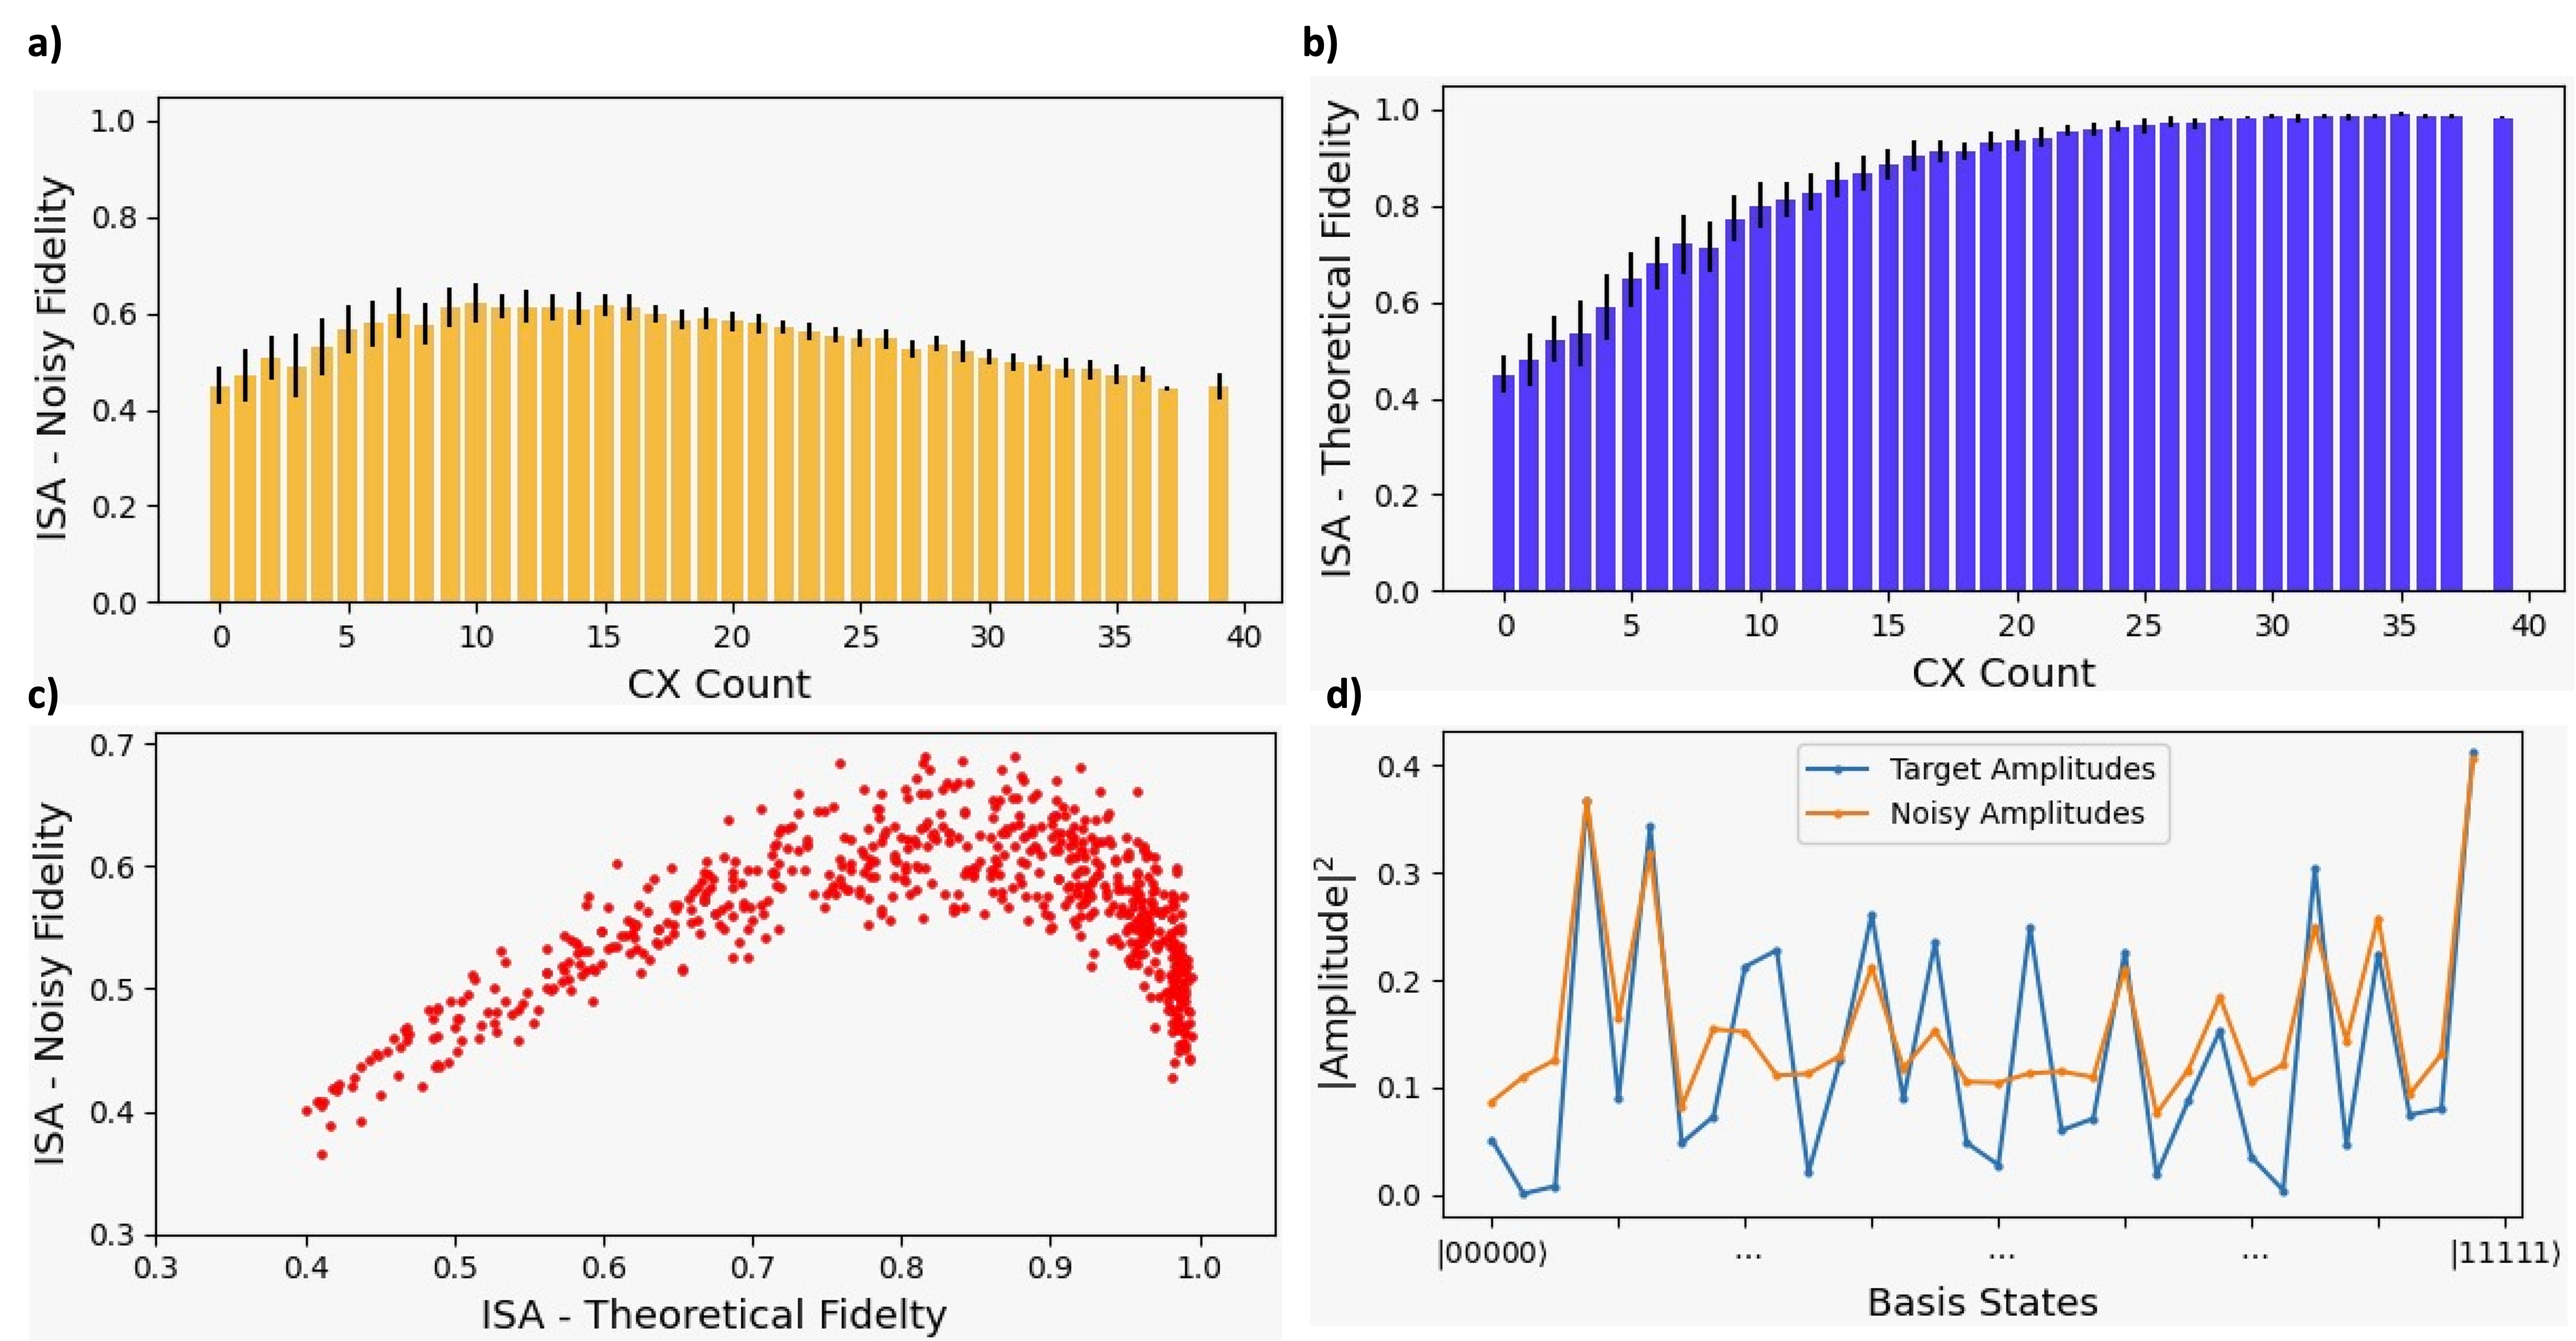
\includegraphics[width=0.95\linewidth]{main/figs/fig3.png}
\caption{Theoretical fidelity, noisy fidelity, and CX gate count for ISA on randomly
sampled five-qubit states on imbq\_melbourne quantum hardware. a)Noisy fidelity versus CX gate count across all 100 states. The error bars represent one
standard deviation at each CX gate count. The bar chart shows that the noisy fidelity
peaks around 10 CX gates. b) theoretical fidelity
versus CX gate count across all 100 states. The error bars represent one standard
deviation at each CX count. The graph shows that as CX gate count increases,
theoretical fidelity increases. c) Noisy fidelity
versus theoretical fidelity. The scatter plot shows that increasing theoretical fidelity
increases the noisy fidelity up to a theoretical fidelity of 0.8, then the curve
inverts and the two quantities become negatively correlated. d) Target state and prepared state amplitude vs basis
vector for the first randomly sampled quantum state. This figure compares the target quantum state
with the quantum state prepared on noisy hardware - while the peaks, corresponding
to large amplitudes, approximately match, the valleys corresponding to smaller 
amplitudes match less well.}
\label{fig3}
\end{figure}




\subsection{Fidelity of protein-encoded states}
For the second set of experiments, we sampled 20 proteins from the proteome of Homo 
sapiens from the UniProtKB database \cite{consortium2015uniprot}. We embedded these proteins into 
continuous, 1024-dimensional feature vectors using the ProtT5 pre-trained protein 
language model \cite{elnaggar2020prottrans}. We encoded these features into ten-qubit quantum states using 
real amplitude encoding. Classical runtime and CX gate counts were measured using the 
same methods as in the first set of experiments. Theoretical fidelities were also 
determined using the gate sequence outputs of each of the methods. For the third set of experiments, we prepared five-qubit quantum states on Qiskit’s
FakeMelbourneV2 machine, which features a LNN architecture on the first five qubits. 
We sampled 100 five-qubit states uniformly at random. For each state, we ran our ISA 
implementation with target fidelity thresholds ranging from 0.4 to 0.95 in increments 
of 0.05, then included an additional target fidelity threshold of 0.98, for a total 
of 13 trials per state. For each trial, the theoretical fidelity, noisy fidelity, and 
CX gate count were determined. Different target fidelity thresholds for the same 
state sometimes yielded identical gate sequences and corresponding fidelities; these 
duplicates were removed from our results. 

The AA-VQC method needed 71 layers to achieve a minimum average fidelity of 
0.95, corresponding to 320 CX gates. The fidelity of UCG is exactly  1.0, as 
it's an exact state preparation method rather than an approximation. Figure \ref{fig2}b
shows that the number of CX gates needed for the VQC-based methods is 
approximately $0.3N = 307.2$, which is consistent with the CX gate counts
reported for AA-VQC and ADAPT-VQE methods in Table 2. In addition, the CX gate
counts for ISA and UCG in Table 2 are consistent with those shown in Table 1.
Thus, all methods returned similar gate counts for both protein-encoded states
and randomly generated states. In addition, the classical runtimes shown in
Table 2 for UCG and ISA methods are consistent with those presented 
in Figure \ref{fig2}a. In addition, despite the timeout for the VQC-based methods at ten 
qubits, as shown in Figure \ref{fig2}, the classical runtime values are consistent with 
the general trend of pure VQC being several orders of magnitude slower than ISA 
and ADAPT-VQE being an order of magnitude slower than AA-VQC. Thus, the 
classical runtime results for protein-encoded states are consistent with those 
for general quantum states.

\begin{table}[h]
\centering
\caption{Average number of CX gates used to prepare 100 randomly generated quantum states versus number of qubits. The values in the ISA and ADAPT-VQE column show two decimal digits, since the number of CX gates used varied across quantum states. By contrast, the values for the UCG column were theoretically determined, and are therefore whole numbers. In addition, the values for AA-VQC were calculated by finding the minimum number of CX gates corresponding to an average fidelity of 0.95 - these are also whole numbers.}
\begin{tabular}{|c||c|c|c|c|}
\hline
Number of Qubits & ISA & UCG & ADAPT-VQE & AA-VQC\\
\hline
5 & 24.08 & 55 & 13.67 & 14 \\
6 & 60.98 & 121 & 25.97 & 28 \\
7 & 143.46 & 251 & 47.96 & 48 \\
8 & 319.02 & 509 & 88.76 & 91 \\
9 & 689.32 & 1023 & 164.22 & 180 \\
10 & 1439.6 & 2049 & TIMEOUT & TIMEOUT \\
11 & 2952.66 & 4099 & & \\
12 & 5991.51 & 8197 & & \\
13 & 12123.3 & 16391 & & \\
14 & 24538 & 32777 & & \\
\hline
\end{tabular}
\end{table}




\subsection{Computational performance}
Figure \ref{fig2}a shows the average classical runtime versus the number of qubits for each
method. For all numbers of qubits tested, the ISA implementation ran the fastest,
however, the ISA method's classical runtime increases faster with qubit number
compared to the UCG method. Thus, the UCG method is expected to be faster than ISA
for more than 14 qubits. Both methods were orders of magnitude faster than the
variational methods. This reflects the intense computational cost incurred by
the gate optimization procedures.

\begin{table}[h]
\centering
\caption{Minimum CX gate count and classical runtime to achieve 0.95 ideal
fidelity for each state preparation method. Each result is an average across 
the 20 trials of preparing distinct protein-encoded quantum states.}
\begin{tabular}{|c|c|c|}
\hline
Method & CX gate count & Classical Runtime \\
\hline
ISA & 1422.3 & $6.420 \times 10^{-2}$ \\
UCG & 2049 & $1.801 \times 10^0$ \\
ADAPT-VQE & 286.0 & $6.424 \times 10^3$ \\
AA-VQC & 320 & $4.895 \times 10^1$ \\
\hline
\end{tabular}
\end{table}

Table 1 shows the average number of CX gates used by each method as a function of the 
number of qubits. The UCG method uses the most CX gates. The ISA method uses somewhat 
fewer CX gates, while the variational methods use the fewest CX gates. The 
variational methods far outperform the non-variational methods in this regard, 
demonstrating the effectiveness of the variational optimization procedure. That said, 
the ISA method is shown to outperform the UCG method without any variational angle 
tuning procedure, indicating that ISA is able to find good QSP gate sequences.

The number of free parameters in the quantum circuit is proportional to the number of 
CX gates; the number of free parameters needed is proportional to $N$, the number of 
complex amplitudes in the target state. Therefore, we hypothesized that the number of 
CX gates would be approximately proportional to $N$ and try to determine the constant 
factor by graphing CX count divided by $N$ as a function of the number of qubits. If 
the CX count is indeed proportional to $N$, then the graph should approach a
horizontal line for large $n$, asymptotically approaching the constant factor. 
Figure \ref{fig2}b shows the average number of CX gates divided by $N$ as a function of 
qubit number for each method. For our ISA implementation, the curve increases for 
$n < 10$, then stabilizes to around 1.5. Thus, we conclude that our ISA 
implementation uses approximately $1.5N$ CX gates for randomly sampled quantum states.
By contrast, the UCG method is shown to use $2N + 2n - 19$ CX gates, which is $2N$ to
the leading order. Thus, the ISA method is shown to use approximately 25\% fewer CX gates
compared to the UCG method. However, both variational methods stabilize to around
0.3, which is about 5 times better than our ISA implementation, demonstrating the
effectiveness of the (computationally expensive) gate optimization procedure.


\subsection{Simulations with noisy quantum circuits}
Figure \ref{fig3} depicts the theoretical fidelity, noisy fidelity, and CX
gate count from the third set of experiments. Figure
\ref{fig3} shows that as the theoretical fidelity
increases from 0.4 to 0.8, the noisy fidelity increases from 0.4 to 0.6. 
Further increases in theoretical fidelity, however, cause the noisy fidelity 
to decrease. This inverse-U shaped correlation between the noisy fidelity and 
the theoretical fidelity is expected because increasing target fidelity 
increases the CX gate count; at first, CX gates improve the quality of the 
prepared state, but beyond a point, the marginal utility of a CX gate 
is outweighed by the noise it introduces. Indeed, Figures 
\ref{fig3}a and \ref{fig3}b corroborate these
expectations; while increasing CX gate count monotonically
increases theoretical fidelity, an increase in CX gate count improves noisy
fidelity only up to a peak of 0.68, around 10 CX gates. Figure 
\ref{fig3}d shows that the largest amplitudes in the prepared 
states match the largest amplitudes in the target state, but the smaller
amplitudes match less well. This is a direct consequence of how our 
ISA implementation approximates the target state as the sum of its largest 
amplitudes, then applies corrections for the smaller amplitudes. These 
corrections cannot prepare the smaller amplitudes perfectly, leading to a 
negative correlation between target amplitude magnitude and how closely it 
matches the corresponding amplitude in the prepared state.

\subsection{Hardware considerations and challenges}
For both the random and protein-encoded quantum states, our implementation of the ISA 
framework uses fewer CX gates than exact state preparation methods without incurring 
the variational optimization costs associated with VQC-based methods. However, the 
VQC-based methods are able to prepare quantum states using much fewer CX gates 
compared to the ISA method, and the UCG method is expected to be faster than ISA for 
quantum states on more than 14 qubits. This trend is expected: the less computation 
time a method uses, the lower the quality of its output.

In practice, every CX gate applied introduces hardware noise into the computation. 
Therefore, the design of quantum circuits will require a careful balance between 
using enough CX gates to approximate the desired computation, while not using so many 
CX gates as to corrupt the computation with noise. The ISA framework lends itself to 
a simple method for finding this balance: if too many CX gates are present in the 
state preparation algorithm, delete the gates corresponding to the last ISA 
iteration; if insufficient CX gates are present, perform more sparse approximation 
iterations. This works because each iteration of sparse approximation monotonically 
increases the state preparation fidelity and each additional iteration provides 
diminishing returns on fidelity increase. This idea was demonstrated our noisy 
simulation experiments. Different target fidelity thresholds led to different numbers 
of CX gates, corresponding to a range of different observed preparation fidelities. 
Finding the optimal CX count was reduced to identifying the optimal target fidelity 
threshold along the theoretical versus noisy fidelity plot for that particular state. 
By contrast, creating such a CX gate count vs noisy fidelity curve for a simple VQC 
method would require re-training the quantum circuit at every CX count sampled; for 
large numbers of qubits, this would require many repetitions of the parameter 
optimization procedure, driving up its already-expensive computational cost.

In addition, different quantum hardwares have different qubit connectivity. The 
only hardware-dependent steps in our ISA implementation are enumerating the 
compatible patterns $\{p\}$ and computing $CX(p)$, both of which can be done by an 
analogous breadth first search procedure. Thus, our ISA implementation can be easily 
adapted to different hardware connectivities.
However, the ISA method does face several limitations. Most importantly, our 
implementation of ISA uses four or five times as many CX gates as the VQC-based 
methods. This may cause ISA-generated gate sequences to induce much more noise on 
near term quantum hardware compared to VQC-based methods. This problem may eventually 
be mitigated by future work discovering alternative, easy-to-prepare classes of 
quantum states for approximating dense quantum states, then adapting those 
discoveries towards an improved ISA implementation. In addition, it may be possible 
to incorporate some variational training alongside ISA. However, the cost function, 
training schedule, gradient conditioning, and other things would need to be carefully 
designed to ensure such a hybrid method does not become a worse version of ADAPT-VQE 
or AA-VQC. Another limitation of the ISA method is that it cannot prepare quantum states that 
require extremely high fidelity. This is because the ISA method treats the dense 
target state as a sparse approximate state, therefore, some percentage of the 
fidelity will be lost on every sparse approximation, and chasing down these lost 
details would require many, many more iterations of ISA. That said, many applications 
of QSP, such as machine learning and sampling from probability distributions, require 
only approximate QSP.



\section{Conclusion}

In this work, we introduced a framework for efficient quantum state preparation that addresses key challenges in encoding chemical data like proteins on quantum computers. The proposed Iterated Sparse Approximation (ISA) framework demonstrated several important advantages while balancing the competing demands of gate count optimization, classical computational efficiency, and hardware constraints. The ISA framework achieves approximate quantum state preparation using approximately 25\% fewer CX gates compared to exact methods like UCG, while maintaining compatibility with linear nearest neighbor architectures common in current quantum hardware. This reduction in gate count is crucial for minimizing decoherence effects in near-term quantum devices. The presented results also demonstrated that ISA can prepare quantum states orders of magnitude faster than variational approaches, making it particularly suitable for large-scale applications in protein data encoding. The framework successfully prepared both random uniform quantum states up to 14 qubits and protein-encoded quantum states from the UniProtKB database with high fidelity. The method demonstrated consistent performance across different state preparation tasks, suggesting robust applicability to various quantum computing applications. The limitations of our approach include higher gate counts compared to variational methods and potential challenges in achieving extremely high fidelities. However, these limitations are offset by the method's classical computational efficiency and hardware adaptability. Future work could explore alternative sparse approximation strategies or hybrid approaches incorporating limited variational optimization to further improve gate count efficiency while maintaining the framework's computational advantages.

\section*{Appendix A}


\textit{Lemma A1.} If an X or CX gate $g$ may be applied to a pattern $p$, then for all quantum
    states $\ket{x}$, $g\xi_p\ket{x} = \xi_{g(p)}g\ket{x}$, \forall g \in  \{ X(i), CX(i,j) \vert p_i\neq*, p_j\neq* \}$
\begin{proof}


Define $g(i)$ such that $g\ket{i} = \ket{g(i)}$. Then $g(i) \in I_{g(p)}$ for all
$i \in I_p$. This also implies $g(g(i)) \in I_{g(g(p))}$ for all $g(i) \in I_{g(p)}$.
Applying $g$ twice amounts to the identity transformation in the
context of both patterns and substates, thus, $i \in I_p$ for all $g(i) \in I_{g(p)}$,
implying that $g$ creates a bijection between $I_p$ and $I_{g(p)}$. In addition, given
that X and CX gates on quantum states represent amplitude permutations in the
computational basis, $\braket{g(i)|g|x} = \braket{i|x}$.  It then follows that,
\begin{align}
\label{eq6}
  g\xi_p\ket{x} &= g\sum_{i \in I_p}{{\ket{i}}{\braket{i|x}}} \nonumber \\
  &= \sum_{i \in I_p}{{\ket{g(i)}}{\braket{i|x}}} \nonumber \\
  &= \sum_{i \in I_p}{{\ket{g(i)}}{\braket{g(i)|g|x}}} \nonumber \\
  &= \sum_{j \in I_{g(p)}}{{\ket{j}}{\braket{j|g|x}}} \nonumber \\
  &= \xi_{g(p)}g\ket{x}
\end{align}
\end{proof}

\section*{Appendix B: Refinements for the ISA method}
We describe two optimizations to our implementation of the ISA framework:
refinement by RZ-RY, and retroactive base case reduction.

\subsection*{B.1. Refinement by RZ-RY}
Refinement by RZ-RY seeks to apply approximate quantum state preparation to the
target state $\ket{x}$ without using any CX gates, before applying the ISA
framework. This is done by selecting a zero-bit pattern $p$ such that
$\| \xi_p\ket{x} \|$ is maximized (ties are broken randomly), then applying substate
merging several times to eventually merge $\xi_p\ket{x}$ into $\xi_{p'}\ket{x}$. The
selection procedure resembles the implementation of prepare, but using substate
merging instead of controlled substate merging:
\begin{enumerate}
\item If $p$ is the string of all zeroes, then terminate this procedure.
Otherwise, continue.
\item Construct the set $P$, containing zero-bit patterns $p'$ that differ from
$p$.
\item Select $p'$ such that $\xi_{p'}\ket{x}$ is maximized, with ties broken
randomly.
\item Let $i$ be the index where $p$ and $p'$ differ. If $p[i] = 0$ then merge
$\xi_{p'}\ket{x}$ into $\xi_p\ket{x}$, otherwise, merge $\xi_p\ket{x}$ into $\xi_{p'}\ket{x}$
and update $p = p'$. Return to step 1.
\end{enumerate}

\begin{figure}[h]
\centering
\includegraphics[width=0.95\linewidth]{main/figs/sfig_1.png}
\caption{Quantum circuit components comprising the ISA framework. a) General quantum circuit structure of a single iteration of ISA using a
two-bit pattern $p$. Several iterations of controlled substate merging are
performed on neighboring qubits before a three-qubit state preparation base case
is applied. b) Decomposition of a single iteration of ISA using a two-bit pattern $p$.
The three-qubit state preparation base case is broken down into a distangling
step and a two-qubit state preparation base case. c) General quantum circuit structure for two consecutive iterations of ISA
ending in a three-qubit base case on the same three qubits. Note that the SP2 
base case in the first ISA iteration can be commuted with the controlled substate
merging step in the second ISA iteration. d) General quantum circuit structure for two consecutive iterations of ISA
width the same three-qubit state preparation base case after applying retroactive
base case reduction. The SP2 block from Figure 4 is merged with the later SP3
block, saving 1 CX gate.}
\label{sfig1}
\end{figure}

\subsection*{B.2. Retroactive Base Case Reduction}
When a two-bit pattern $p$ is chosen in the select step, the corresponding quantum
circuit takes on the structure shown in Figure \ref{sfig1}a. The three-qubit QSP step can be broken into two steps: disentangling the third 
qubit and two-qubit state preparation on the remaining two qubits, as shown in 
Figure \ref{sfig1}b. However, if two consecutive iterations of ISA both selected a
two-bit pattern and those 
two patterns had their `$*$' characters on the same two qubits, the resulting 
quantum circuit would have the structure shown in Figure \ref{sfig1}c. Then,
the part of the quantum circuit enclosed in dotted lines first performs 
two-qubit state preparation on the lower two qubits, then performs three-qubit 
state preparation on all three relevant qubits. These two transformations have 
the net effect of transforming the three-qubit substate to $\ket{\mathbf{0}}$ and can
instead be replaced by a single three-qubit state preparation routine. This
procedure saves the one CX gate used by the two-qubit state preparation base
case.

\section*{Appendix C: Optimal, exact three-qubit state preparation}
Optimal, exact three-qubit state preparation has been studied in the 
literature \cite{PhysRevA.77.032320}; our specific implementation requires
three steps, called ``D1'', ``D2'', and ``SP2''. Let the target state be
\begin{equation}
\ket{x} = \sum_{i, j, k \in \{0, 1\}}{a_{ijk}\ket{ijk}}.
\end{equation}
Step D1 applies a single-qubit rotation, then CX(0, 1), then another single-qubit
rotation, resulting in the state
\begin{equation}
\ket{y} = \sum_{i, j, k \in \{0, 1\}}{b_{ijk}\ket{ijk}},
\end{equation}
such that
\begin{equation}
\frac{b_{110}}{b_{010}} = \frac{b_{111}}{b_{011}} \quad 
  and \quad \frac{b_{100}}{b_{000}} = \frac{b_{101}}{b_{001}}.
\end{equation}
Next, step D2 uses a single-qubit rotation, CX(1, 2), and another single-qubit
rotation to transform $\ket{y}$ into a two-qubit state
\begin{equation}
\ket{z} = \sum_{j, k \in \{0, 1\}}{c_{jk}\ket{0jk}}.
\end{equation}
Finally, step SP2 implements two-qubit state preparation on this state using one
CX gate and several single-qubit rotations. We describe each of these steps in detail,
starting with SP2 and D2. Then, we briefly discuss the decomposition of uniformly
controlled single-qubit rotations before concluding with a description of D1.

\subsection*{C.1. SP2}
Starting from the state 
\begin{equation}
\ket{z} = \sum_{j, k \in \{0, 1\}}{c_{jk}\ket{0jk}},
\end{equation}
we rotate merge $c_{001}\ket{001}$ into $c_{000}\ket{000}$, leading to the state:
\begin{equation}
\ket{z'} = c'_{000}\ket{000} + c'_{010}\ket{010} + c'_{011}\ket{011}.
\end{equation}
Next, $c'_{011}\ket{011}$ is controlled rotate merged into $c'_{010}\ket{010}$. This
results in a one-qubit state that can be prepared using a single-qubit rotation gate.

\subsection*{C.2. Step D2}
Starting from the state
\begin{equation}
\ket{y} = \sum_{i, j, k \in \{0, 1\}}{b_{ijk}\ket{ijk}},
\end{equation}
 we rotate merge $b_{100}\ket{100}$ into $b_{000}\ket{000}$. The pre-condition
\begin{equation}
\frac{b_{100}}{b_{000}} = \frac{b_{101}}{b_{001}}
\end{equation}
ensures that this procedure also merges $b_{101}\ket{101}$ into $b_{001}\ket{001}$.
This results in the state:
\begin{align}
\ket{y} = \sum_{i, j, k \in \{0, 1\}}{b'_{ijk}\ket{ijk}} \nonumber \\
\text{such that} \quad b'_{100}, b'_{101} = 0
\end{align}
In addition, the RZ and RY gate were applied to qubit 2, therefore, the equality
\begin{equation}
\frac{b_{110}}{b_{010}} = \frac{b_{111}}{b_{011}}
\end{equation}
is preserved after the transformation.
\begin{equation}
\frac{b'_{110}}{b'_{010}} = \frac{b'_{111}}{b'_{011}}
\end{equation}
Next, $b'_{110}\ket{110}$ is controlled rotate merged into $b'_{010}\ket{010}$. The
equality
\begin{equation}
\frac{b'_{110}}{b'_{010}} = \frac{b'_{111}}{b'_{011}}
\end{equation}
ensures that $b'_{111}\ket{111}$ is also merged into $b'_{011}\ket{011}$ by this
process. The previous step zeroed out the $\ket{100}$ and $\ket{101}$ basis vectors;
this step zeroed out the $\ket{110}$ and $\ket{111}$ basis vectors. Therefore, the
result of these transformations is a two-qubit state:
\begin{equation}
\ket{z} = \sum_{j, k \in \{0, 1\}}{c_{jk}\ket{0jk}}.
\end{equation}
\subsection*{C.3. Decomposing Uniformly Controlled Single-Qubit Rotations}
In this section, we describe the set of uniformly controlled single-qubit rotations 
with one control qubit that can be decomposed into one CX gate and single-qubit 
rotations. In addition, we give a procedure for their decomposition. These 
constructions will be necessary for the construction of step D1 for optimal, exact 
three-qubit state preparation.

\begin{figure}[h]
\centering
\includegraphics[width=0.6\linewidth]{main/figs/sfig_2.png}
\caption{a) The circuit block used in ADAPT-VQE for state preparation. The operator
pool was generated by translating this block across different pairs of 
adjacent qubits. Each operator contains four parameters, one for each rotation.
All four rotation angles were initialized to zero. b) Target decomposition of the uniformly controlled single-qubit rotation with one control qubit}
\label{sfig2}
\end{figure}

For simplicity, let the control qubit be qubit 1, let the target qubit be qubit 0. 
Suppose the desired gate applies $a$ if the control qubit is 0, applies $b$ 
otherwise. Then the desired gate has matrix form 
\begin{equation}
\begin{bmatrix}a&0\\0&b\end{bmatrix}.
\end{equation}
We wish to decompose this transformation into a quantum circuit of the form shown in
Figure \ref{sfig2}b.




These gates, together, take the matrix form
\begin{equation}
\begin{bmatrix}v&0\\0&v\end{bmatrix}
\begin{bmatrix}I&0\\0&X\end{bmatrix}
\begin{bmatrix}u&0\\0&u\end{bmatrix},
\end{equation}
This requires some $u$ and $v$ to exist such that $a = vu$ and $b = vXu$. Then
\begin{equation}
ab^\dagger = (vu)(vXu)^\dagger = vXv^\dagger,
\end{equation}
which implies that $ab^\dagger$ must have the same eigenvalues, $\pm 1$, as $X$.
This condition is both necessary and sufficient for the uniformly controlled rotation
to be decomposable into the quantum circuit shown. Indeed, if $ab^\dagger$ has the
same eigenvalues as $X$, then we can compute $v$ by diagonalization, then compute
$u = v^\dagger a$. Finally, $u$ and $v$ can be decomposed to RY and RZ gates using
ZYZ decomposition.

\subsection*{C.4. Step D1}
Step D1 is implemented using a uniformly controlled single-qubit rotation, with
qubit 0 as the control, qubit 1 as the target. To implement D1, we construct
single-qubit operations $a$ and $b$ such that applying
$\begin{bmatrix}a&0\\0&b\end{bmatrix}$ to $\ket{x}$ leads to the state
\begin{equation}
\ket{y} = \sum_{i, j, k \in \{0, 1\}}{b_{ijk}\ket{ijk}},
\end{equation}
such that
\begin{equation}
\frac{b_{110}}{b_{010}} = \frac{b_{111}}{b_{011}} 
  \text{ and } \frac{b_{100}}{b_{000}} = \frac{b_{101}}{b_{001}}
\end{equation}
In addition, we perform this construction such that $ab^\dagger$ has eigenvalues
$\pm 1$ to ensure the transformation can be implemented using only one CX gate.

We parameterize $a$ and $b$ as:
\begin{align}
a &= e^{i\phi_g}\begin{bmatrix}cos(\theta_a)&-sin(\theta_a)e^{i\phi_a}\\
  sin(\theta_a)e^{i\alpha_a}&cos(\theta_a)e^{i(\alpha_a + \phi_a)}\end{bmatrix} 
  \nonumber \\
b &= \begin{bmatrix}cos(\theta_b)&-sin(\theta_b)e^{i\phi_b}\\
  sin(\theta_b)e^{i\alpha_b}&cos(\theta_b)e^{i(\alpha_b + \phi_b)}\end{bmatrix}
\end{align}
Then, we can express the $b_{ijk}$ coefficients of $\ket{y}$ in terms of
$\phi_g$, $\theta_a$, $\alpha_a$, $\phi_a$, $\theta_b$, $\alpha_b$, $\phi_b$,
and the $a_{ijk}$ coefficients of $\ket{x}$:

\begin{align}
b_{000} &= e^{i\phi_g}(cos(\theta_a)a_{000} + sin(\theta_a)e^{i\phi_a}a_{010}) 
  \nonumber \\
b_{010} &= e^{i(\alpha_a + \phi_g)}(-sin(\theta_a)a_{000} +
  cos(\theta_a)e^{i\phi_a}a_{010}) \nonumber \\
b_{100} &= e^{i\phi_g}(cos(\theta_a)a_{100} + sin(\theta_a)e^{i\phi_a}a_{110}) 
  \nonumber \\
b_{110} &= e^{i(\alpha_a + \phi_g)}(-sin(\theta_a)a_{100} +
  cos(\theta_a)e^{i\phi_a}a_{110}) \nonumber \\
b_{001} &= cos(\theta_b)a_{001} + sin(\theta_b)e^{i\phi_b}a_{011} \nonumber \\
b_{011} &= e^{i\alpha_b}(-sin(\theta_b)a_{001} + cos(\theta_b)e^{i\phi_b}a_{011}) 
  \nonumber \\
b_{101} &= cos(\theta_b)a_{101} + sin(\theta_b)e^{i\phi_b}a_{111} \nonumber \\
b_{111} &= e^{i\alpha_b}(-sin(\theta_b)a_{101} + cos(\theta_b)e^{i\phi_b}a_{111})
  \nonumber \\
\end{align}
Then the constraints
\begin{equation}
\frac{b_{110}}{b_{010}} = \frac{b_{111}}{b_{011}} 
  \text{ and }\frac{b_{100}}{b_{000}} = \frac{b_{101}}{b_{001}}
\end{equation}
Can be written as:

\begin{align}
\frac{e^{i(\alpha_a + \phi_g)}(-sin(\theta_a)a_{100} + cos(\theta_a)e^{i\phi_a}a_{110})}{e^{i(\alpha_a + \phi_g)}(-sin(\theta_a)a_{000} + cos(\theta_a)e^{i\phi_a}a_{010})} &= 
\frac{e^{i\alpha_b}(-sin(\theta_b)a_{101} + cos(\theta_b)e^{i\phi_b}a_{111})}{e^{i\alpha_b}(-sin(\theta_b)a_{001} + cos(\theta_b)e^{i\phi_b}a_{011})} \nonumber \\
\frac{e^{i\phi_g}(cos(\theta_a)a_{100} + sin(\theta_a)e^{i\phi_a}a_{110})}{e^{i\phi_g}(cos(\theta_a)a_{000} + sin(\theta_a)e^{i\phi_a}a_{010})} &= \frac{cos(\theta_b)a_{101} + sin(\theta_b)e^{i\phi_b}a_{111}}
{cos(\theta_b)a_{001} + sin(\theta_b)e^{i\phi_b}a_{011}}
\end{align}

The $e^{i\alpha_a}$, $e^{i\alpha_b}$, $e^{i\phi_g}$ terms cancel out,
making $\phi_g$, $\alpha_a$, and $\alpha_b$ free parameters. Multiplying out
the denominators, dividing by $cos(\theta_a)cos(\theta_b)$, and re-arranging the
terms gives:

\begin{align}
Atan(\theta_a)tan(\theta_b) + Btan(\theta_a)e^{i\phi_b} + Ctan(\theta_b)e^{i\phi_a} + De^{i(\phi_a + \phi_b)} = 0 \nonumber \\
A - Btan(\theta_b)e^{i\phi_b} - Ctan(\theta_a)e^{i\phi_a} + Dtan(\theta_a)tan(\theta_b)e^{i(\phi_a + \phi_b)} = 0
\end{align}

where
\begin{align}
A &= a_{100}a_{001} - a_{000}a_{101}\nonumber \\
B &= a_{100}a_{011} - a_{000}a_{111}\nonumber \\
C &= a_{110}a_{001} - a_{010}a_{101}\nonumber \\
D &= a_{110}a_{011} - a_{010}a_{111}
\end{align}

Dividing the first equation by $e^{i(\phi_a + \phi_b)}$ and taking its conjugate
results in the following system of equations:

\begin{align}
A^*tan(\theta_a)tan(\theta_b)e^{i(\phi_a + \phi_b)} + B^*tan(\theta_a)e^{i\phi_a} + C^*tan(\theta_b)e^{i\phi_b} + D^* = 0 \nonumber \\
A - Btan(\theta_b)e^{i\phi_b} - Ctan(\theta_a)e^{i\phi_a} + Dtan(\theta_a)tan(\theta_b)e^{i(\phi_a + \phi_b)} = 0.
\end{align}

Performing the substitution
\begin{align}
x = tan(\theta_a)e^{i\phi_a} \nonumber \\
y = tan(\theta_b)e^{i\phi_b}
\end{align}

Results in the system of equations:
\begin{align}
A^*xy + B^*x + C^*y + D^* = 0 \nonumber \\
A - By - Cx + Dxy = 0
\end{align}

Which can be solved by substitution. Once $x$ and $y$ are known,
$\theta_a$, $\theta_b$, $\phi_a$, $\phi_b$ can be determined.

Next, the constraint on the eigenvalues of $ab^\dagger$ needs to be satisfied.
Using the same parameterization as before, we can write:
\begin{align}
a &= e^{i\phi_g}\begin{bmatrix}cos(\theta_a)&-sin(\theta_a)e^{i\phi_a}\\
  sin(\theta_a)e^{i\alpha_a}&cos(\theta_a)e^{i(\phi_a + \alpha_a)}\end{bmatrix}
  = e^{i\phi_g}\begin{bmatrix}1&0\\0&e^{i\alpha_a}\end{bmatrix}\begin{bmatrix}
  cos(\theta_a)&-sin(\theta_a)e^{i\phi_a}\\sin(\theta_a)&cos(\theta_a)e^{i\phi_a}
  \end{bmatrix} \nonumber \\
b &= \begin{bmatrix}cos(\theta_b)&-sin(\theta_b)e^{i\phi_b}\\
  sin(\theta_b)e^{i\alpha_b}&cos(\theta_b)e^{i(\phi_b + \alpha_b)}\end{bmatrix}
  = \begin{bmatrix}1&0\\0&e^{i\alpha_b}\end{bmatrix}\begin{bmatrix}cos(\theta_b)
  &-sin(\theta_b)e^{i\phi_b}\\sin(\theta_b)&cos(\theta_b)e^{i\phi_b}\end{bmatrix}
  \nonumber \\
ab^\dagger &= e^{i\phi_g}\begin{bmatrix}1&0\\0&e^{i\alpha_a}\end{bmatrix}\left(
  \begin{bmatrix}cos(\theta_a)&-sin(\theta_a)e^{i\phi_a}\\
  sin(\theta_a)&cos(\theta_a)e^{i\phi_a}\end{bmatrix}\begin{bmatrix}
  cos(\theta_b)&-sin(\theta_b)e^{i\phi_b}\\sin(\theta_b)
  &cos(\theta_b)e^{i\phi_b}\end{bmatrix}^\dagger\right)\begin{bmatrix}1&0\\
  0&e^{i\alpha_b}\end{bmatrix}^\dagger \label{abt}
\end{align}

The two matrices between the parentheses in Eq. (\ref{abt}) are unitary matrices, thus, their
product is a unitary matrix and can be expressed as
\begin{equation}
\begin{bmatrix}cos(\theta_a)&-sin(\theta_a)e^{i\phi_a}\\
  sin(\theta_a)&cos(\theta_a)e^{i\phi_a}\end{bmatrix}\begin{bmatrix}
  cos(\theta_a)&-sin(\theta_a)e^{i\phi_a}\\sin(\theta_a)
  &cos(\theta_a)e^{i\phi_a}\end{bmatrix}^\dagger = 
  e^{i\alpha_g}\begin{bmatrix}cos(\theta)&-sin(\theta)e^{i\phi}\\
  sin(\theta)e^{i\alpha}&cos(\theta)e^{i(\alpha + \phi)}\end{bmatrix}
\end{equation}
for some $\alpha_g$, $\alpha$, $\phi$, and $\theta$. Then, we can write
\begin{align}
ab^\dagger &= e^{i\phi_g}\begin{bmatrix}1&0\\0&e^{i\alpha_a}\end{bmatrix}
  e^{i\alpha_g}\begin{bmatrix}cos(\theta)&-sin(\theta)e^{i\phi}\\
  sin(\theta)e^{i\alpha}&cos(\theta)e^{i(\alpha + \phi)}\end{bmatrix}
  \begin{bmatrix}1&0\\0&e^{i\alpha_b}\end{bmatrix}^\dagger \nonumber \\
 &= e^{i(\phi_g + \alpha_g)}\begin{bmatrix}cos(\theta)&-sin(\theta)
  e^{i(\phi - \alpha_b)}\\sin(\theta)e^{i(\alpha + \alpha_a)}
  &cos(\theta)e^{i(\phi + \alpha + \alpha_a - \alpha_b)}\end{bmatrix}
\end{align}

The characteristic polynomial of this matrix is:
\begin{align}
p(t) &= (cos(\theta)e^{i(\phi_g + \alpha_g)} - t)
(cos(\theta)e^{i(\phi + \alpha + \alpha_a - \alpha_b + \phi_g + \alpha_g)} - t) \nonumber \\
&\quad \quad - (-sin(\theta)e^{i(\phi - \alpha_b + \phi_g + \alpha_g)})
  (sin(\theta)e^{i(\alpha - \alpha_a + \phi_g + \alpha_g)}) \nonumber \\
 &= t^2 - e^{i(\phi_g + \alpha_g)}cos(\theta)(1 + e^{i(\phi + \alpha + \alpha_a - \alpha_b)})t 
  + cos(\theta)^2e^{i(2(\phi_g + \alpha_g) + \phi + \alpha + \alpha_a - \alpha_b)} \nonumber \\
  &\quad \quad+ sin(\theta)^2e^{i(2(\phi_g + \alpha_g) + \phi + \alpha + \alpha_a - \alpha_b)} \nonumber \\
 &= t^2 - e^{i(\phi_g + \alpha_g)}cos(\theta)(1 + e^{i(\phi + \alpha + \alpha_a - \alpha_b)})t + e^{2i(\phi_g + \alpha_g)}e^{i(\phi + \alpha + \alpha_a - \alpha_b)}
\end{align}
We require the eigenvalues to be $\pm 1$, so the characteristic polynomial must
be equal to $t^2 - 1$. This requires:
\begin{align}
e^{i(\phi_g + \alpha_g)}cos(\theta)(1 + e^{i(\phi + \alpha + \alpha_a - \alpha_b)}) = 0 \nonumber \\
e^{2i(\phi_g + \alpha_g)}e^{i(\phi + \alpha + \alpha_a - \alpha_b)} = -1
\end{align}
Solving these equations gives:
\begin{align}
\phi + \alpha + \alpha_a - \alpha_b = \pi \nonumber \\
\phi_g + \alpha_g = 0
\end{align}
Therefore, we set $\phi_g = -\alpha_g$, $\alpha_a = \pi - \phi - \alpha$, and
$\alpha_b = 0$ to ensure that $ab^\dagger$ is similar to $X$. Now, all the
parameters in $a$ and $b$ are specified, and the procedure from the previous
section can be used to compute the gate sequence implementing the desired
transformation. This concludes the description of each individual step in our
linear nearest neighbors implementation of optimal, exact three-qubit state
preparation.

\subsection*{C.5. CX gate count for UCG Exact Method on LNN Architecture}
Bergholm et al \cite{bergholm2005quantum} showed that exact QSP on $n$ qubits can be reduced to a
sequence of $n$ uniformly controlled single-qubit gates, where the $k$th gate
uses qubits $[0...n-1-k]$ as the controls, and qubit $n-k$ as the target. 
The last UCG is a single-qubit rotation on qubit 0. Next, the authors showed
that, on LNN architectures, a uniformly controlled single-qubit gate using
controls $[0...c-1]$ and target qubit $c$ can be implemented, up to a diagonal
gate, as
\begin{equation}
\text{UCG}(c) = \prod_{i = 0}^{2^c - 1}{\text{CX chain}(c - 1 - z(i), c)U(i)},
\label{UCGdef}
\end{equation}
for some choice of single-qubit rotations $U(i)$, where $z(i)$ is the number of
trailing zeroes in the binary representation of $i$ (define $z(0) = c - 1$)
and CX chain($i$, $j$) is a sequence of CX gates:
\begin{align}
\text{CX chain}(i, j) = &CX(i, i + 1)CX(i + 1, i + 2)...CX(j - 2, j - 1)
CX(j - 1, j) \nonumber \\
&CX(j - 2, j - 1)...CX(i + 1, i + 2)CX(i, i + 1)
\end{align}
The number of CX gates in CX chain($i$, $j$) is $2(j - i) - 1$. Then, the number
of CX gates needed to implement UCG($c$) is
\begin{align}
\text{CX count(UCG($c$))} &= \sum_{i = 0}^{2^c - 1}{(2(1 + z(i)) - 1)} \nonumber \\
&=\sum_{i = 0}^{2^c - 1}{(2z(i) + 1)} \nonumber \\
&=2^c + 2\sum_{i = 0}^{2^c - 1}{z(i)}.
\end{align}
Since $i$ takes on all non-negative integers with $c$ bits inthe sum, there are
$2^{c-m-1}$ instances where $z(i) = m$, for $0 \leq m \leq c - 2$. However, 
$m = c - 1$ will show up twice because $z(0)$ is defined to be $c - 1$. Then,
\begin{align}
\sum_{i = 0}^{2^c - 1}{z(i)} = \sum_{m = 0}^{c - 2}{m2^{c - m - 1} + 2(c - 1)} 
= 2^c - 2 \nonumber \\
\text{CX count(UCG($c$))} = 2^c + 2(2^c - 2) = 3 \times 2^c - 4.
\end{align}
This would be the number of CX gates required to implement UCG($c$) on an LNN
architecture, however, \cite{bergholm2005quantum} introduces an optimization: by swapping qubits $c$
and $c - 1$, all of the $\text{CX chain}(c - 1 - z(i), c)$ terms in 
Eq. (\ref{UCGdef}), where $c - 1 - z(i) < c - 1$, become 
$\text{CX chain}(c - 1 - z(i), c - 1)$. This saves 2 CX gates for each of those
terms. In addition, for the CX chains where $c - 1 - z(i) = c - 1$, the 
$\text{CX chain}(c - 1 - z(i), c)$ term becomes CX chain($c - 1$, $c$), which is
the same thing. The swapping procedure costs 6 CX gates (3 to swap the qubits, 3
to swap back at the end), but it saves 2 CX gates for each term where 
$c - 1 - z(i) < c - 1 \implies z(i) > 0$. There are $2^{c - 1}$ such terms, for
a net savings of $2^c - 6$ CX gates. Thus,
\begin{equation}
\text{CX count, optimized(UCG($c$))} = 3 \times 2^c - 4 - (2^c - 6) 
  = 2 \times 2^c + 2.
\end{equation}
We introduce one additional optimization: the UCG(2), UCG(1), and UCG(0) gates
at the end can be replaced by exact, optimal three-qubit state preparation. Then,
we can compute the total number of CX gates required to prepare an $n$-qubit
quantum state ($n > 3$) using the UCG method:
\begin{align}
\text{CX count, UCG on $n$ qubits} = 3 + \sum_{k = 3}^{n - 1}{(2 \times 2^k + 2)}
\nonumber \\
= 3 + 2(2^n - 8) + 2(n - 3) = 2 \times 2^n + 2n - 19.
\end{align}


\clearpage

\begin{left}
    \textbf{References}
\end{left}
\printbibliography[heading=none]

% \clearpage
% \section*{Appendix A}


\textit{Lemma A1.} If an X or CX gate $g$ may be applied to a pattern $p$, then for all quantum
    states $\ket{x}$, $g\xi_p\ket{x} = \xi_{g(p)}g\ket{x}$, \forall g \in  \{ X(i), CX(i,j) \vert p_i\neq*, p_j\neq* \}$
\begin{proof}


Define $g(i)$ such that $g\ket{i} = \ket{g(i)}$. Then $g(i) \in I_{g(p)}$ for all
$i \in I_p$. This also implies $g(g(i)) \in I_{g(g(p))}$ for all $g(i) \in I_{g(p)}$.
Applying $g$ twice amounts to the identity transformation in the
context of both patterns and substates, thus, $i \in I_p$ for all $g(i) \in I_{g(p)}$,
implying that $g$ creates a bijection between $I_p$ and $I_{g(p)}$. In addition, given
that X and CX gates on quantum states represent amplitude permutations in the
computational basis, $\braket{g(i)|g|x} = \braket{i|x}$.  It then follows that,
\begin{align}
\label{eq6}
  g\xi_p\ket{x} &= g\sum_{i \in I_p}{{\ket{i}}{\braket{i|x}}} \nonumber \\
  &= \sum_{i \in I_p}{{\ket{g(i)}}{\braket{i|x}}} \nonumber \\
  &= \sum_{i \in I_p}{{\ket{g(i)}}{\braket{g(i)|g|x}}} \nonumber \\
  &= \sum_{j \in I_{g(p)}}{{\ket{j}}{\braket{j|g|x}}} \nonumber \\
  &= \xi_{g(p)}g\ket{x}
\end{align}
\end{proof}

\section*{Appendix B: Refinements for the ISA method}
We describe two optimizations to our implementation of the ISA framework:
refinement by RZ-RY, and retroactive base case reduction.

\subsection*{B.1. Refinement by RZ-RY}
Refinement by RZ-RY seeks to apply approximate quantum state preparation to the
target state $\ket{x}$ without using any CX gates, before applying the ISA
framework. This is done by selecting a zero-bit pattern $p$ such that
$\| \xi_p\ket{x} \|$ is maximized (ties are broken randomly), then applying substate
merging several times to eventually merge $\xi_p\ket{x}$ into $\xi_{p'}\ket{x}$. The
selection procedure resembles the implementation of prepare, but using substate
merging instead of controlled substate merging:
\begin{enumerate}
\item If $p$ is the string of all zeroes, then terminate this procedure.
Otherwise, continue.
\item Construct the set $P$, containing zero-bit patterns $p'$ that differ from
$p$.
\item Select $p'$ such that $\xi_{p'}\ket{x}$ is maximized, with ties broken
randomly.
\item Let $i$ be the index where $p$ and $p'$ differ. If $p[i] = 0$ then merge
$\xi_{p'}\ket{x}$ into $\xi_p\ket{x}$, otherwise, merge $\xi_p\ket{x}$ into $\xi_{p'}\ket{x}$
and update $p = p'$. Return to step 1.
\end{enumerate}

\begin{figure}[h]
\centering
\includegraphics[width=0.95\linewidth]{main/figs/sfig_1.png}
\caption{Quantum circuit components comprising the ISA framework. a) General quantum circuit structure of a single iteration of ISA using a
two-bit pattern $p$. Several iterations of controlled substate merging are
performed on neighboring qubits before a three-qubit state preparation base case
is applied. b) Decomposition of a single iteration of ISA using a two-bit pattern $p$.
The three-qubit state preparation base case is broken down into a distangling
step and a two-qubit state preparation base case. c) General quantum circuit structure for two consecutive iterations of ISA
ending in a three-qubit base case on the same three qubits. Note that the SP2 
base case in the first ISA iteration can be commuted with the controlled substate
merging step in the second ISA iteration. d) General quantum circuit structure for two consecutive iterations of ISA
width the same three-qubit state preparation base case after applying retroactive
base case reduction. The SP2 block from Figure 4 is merged with the later SP3
block, saving 1 CX gate.}
\label{sfig1}
\end{figure}

\subsection*{B.2. Retroactive Base Case Reduction}
When a two-bit pattern $p$ is chosen in the select step, the corresponding quantum
circuit takes on the structure shown in Figure \ref{sfig1}a. The three-qubit QSP step can be broken into two steps: disentangling the third 
qubit and two-qubit state preparation on the remaining two qubits, as shown in 
Figure \ref{sfig1}b. However, if two consecutive iterations of ISA both selected a
two-bit pattern and those 
two patterns had their `$*$' characters on the same two qubits, the resulting 
quantum circuit would have the structure shown in Figure \ref{sfig1}c. Then,
the part of the quantum circuit enclosed in dotted lines first performs 
two-qubit state preparation on the lower two qubits, then performs three-qubit 
state preparation on all three relevant qubits. These two transformations have 
the net effect of transforming the three-qubit substate to $\ket{\mathbf{0}}$ and can
instead be replaced by a single three-qubit state preparation routine. This
procedure saves the one CX gate used by the two-qubit state preparation base
case.

\section*{Appendix C: Optimal, exact three-qubit state preparation}
Optimal, exact three-qubit state preparation has been studied in the 
literature \cite{PhysRevA.77.032320}; our specific implementation requires
three steps, called ``D1'', ``D2'', and ``SP2''. Let the target state be
\begin{equation}
\ket{x} = \sum_{i, j, k \in \{0, 1\}}{a_{ijk}\ket{ijk}}.
\end{equation}
Step D1 applies a single-qubit rotation, then CX(0, 1), then another single-qubit
rotation, resulting in the state
\begin{equation}
\ket{y} = \sum_{i, j, k \in \{0, 1\}}{b_{ijk}\ket{ijk}},
\end{equation}
such that
\begin{equation}
\frac{b_{110}}{b_{010}} = \frac{b_{111}}{b_{011}} \quad 
  and \quad \frac{b_{100}}{b_{000}} = \frac{b_{101}}{b_{001}}.
\end{equation}
Next, step D2 uses a single-qubit rotation, CX(1, 2), and another single-qubit
rotation to transform $\ket{y}$ into a two-qubit state
\begin{equation}
\ket{z} = \sum_{j, k \in \{0, 1\}}{c_{jk}\ket{0jk}}.
\end{equation}
Finally, step SP2 implements two-qubit state preparation on this state using one
CX gate and several single-qubit rotations. We describe each of these steps in detail,
starting with SP2 and D2. Then, we briefly discuss the decomposition of uniformly
controlled single-qubit rotations before concluding with a description of D1.

\subsection*{C.1. SP2}
Starting from the state 
\begin{equation}
\ket{z} = \sum_{j, k \in \{0, 1\}}{c_{jk}\ket{0jk}},
\end{equation}
we rotate merge $c_{001}\ket{001}$ into $c_{000}\ket{000}$, leading to the state:
\begin{equation}
\ket{z'} = c'_{000}\ket{000} + c'_{010}\ket{010} + c'_{011}\ket{011}.
\end{equation}
Next, $c'_{011}\ket{011}$ is controlled rotate merged into $c'_{010}\ket{010}$. This
results in a one-qubit state that can be prepared using a single-qubit rotation gate.

\subsection*{C.2. Step D2}
Starting from the state
\begin{equation}
\ket{y} = \sum_{i, j, k \in \{0, 1\}}{b_{ijk}\ket{ijk}},
\end{equation}
 we rotate merge $b_{100}\ket{100}$ into $b_{000}\ket{000}$. The pre-condition
\begin{equation}
\frac{b_{100}}{b_{000}} = \frac{b_{101}}{b_{001}}
\end{equation}
ensures that this procedure also merges $b_{101}\ket{101}$ into $b_{001}\ket{001}$.
This results in the state:
\begin{align}
\ket{y} = \sum_{i, j, k \in \{0, 1\}}{b'_{ijk}\ket{ijk}} \nonumber \\
\text{such that} \quad b'_{100}, b'_{101} = 0
\end{align}
In addition, the RZ and RY gate were applied to qubit 2, therefore, the equality
\begin{equation}
\frac{b_{110}}{b_{010}} = \frac{b_{111}}{b_{011}}
\end{equation}
is preserved after the transformation.
\begin{equation}
\frac{b'_{110}}{b'_{010}} = \frac{b'_{111}}{b'_{011}}
\end{equation}
Next, $b'_{110}\ket{110}$ is controlled rotate merged into $b'_{010}\ket{010}$. The
equality
\begin{equation}
\frac{b'_{110}}{b'_{010}} = \frac{b'_{111}}{b'_{011}}
\end{equation}
ensures that $b'_{111}\ket{111}$ is also merged into $b'_{011}\ket{011}$ by this
process. The previous step zeroed out the $\ket{100}$ and $\ket{101}$ basis vectors;
this step zeroed out the $\ket{110}$ and $\ket{111}$ basis vectors. Therefore, the
result of these transformations is a two-qubit state:
\begin{equation}
\ket{z} = \sum_{j, k \in \{0, 1\}}{c_{jk}\ket{0jk}}.
\end{equation}
\subsection*{C.3. Decomposing Uniformly Controlled Single-Qubit Rotations}
In this section, we describe the set of uniformly controlled single-qubit rotations 
with one control qubit that can be decomposed into one CX gate and single-qubit 
rotations. In addition, we give a procedure for their decomposition. These 
constructions will be necessary for the construction of step D1 for optimal, exact 
three-qubit state preparation.

\begin{figure}[h]
\centering
\includegraphics[width=0.6\linewidth]{main/figs/sfig_2.png}
\caption{a) The circuit block used in ADAPT-VQE for state preparation. The operator
pool was generated by translating this block across different pairs of 
adjacent qubits. Each operator contains four parameters, one for each rotation.
All four rotation angles were initialized to zero. b) Target decomposition of the uniformly controlled single-qubit rotation with one control qubit}
\label{sfig2}
\end{figure}

For simplicity, let the control qubit be qubit 1, let the target qubit be qubit 0. 
Suppose the desired gate applies $a$ if the control qubit is 0, applies $b$ 
otherwise. Then the desired gate has matrix form 
\begin{equation}
\begin{bmatrix}a&0\\0&b\end{bmatrix}.
\end{equation}
We wish to decompose this transformation into a quantum circuit of the form shown in
Figure \ref{sfig2}b.




These gates, together, take the matrix form
\begin{equation}
\begin{bmatrix}v&0\\0&v\end{bmatrix}
\begin{bmatrix}I&0\\0&X\end{bmatrix}
\begin{bmatrix}u&0\\0&u\end{bmatrix},
\end{equation}
This requires some $u$ and $v$ to exist such that $a = vu$ and $b = vXu$. Then
\begin{equation}
ab^\dagger = (vu)(vXu)^\dagger = vXv^\dagger,
\end{equation}
which implies that $ab^\dagger$ must have the same eigenvalues, $\pm 1$, as $X$.
This condition is both necessary and sufficient for the uniformly controlled rotation
to be decomposable into the quantum circuit shown. Indeed, if $ab^\dagger$ has the
same eigenvalues as $X$, then we can compute $v$ by diagonalization, then compute
$u = v^\dagger a$. Finally, $u$ and $v$ can be decomposed to RY and RZ gates using
ZYZ decomposition.

\subsection*{C.4. Step D1}
Step D1 is implemented using a uniformly controlled single-qubit rotation, with
qubit 0 as the control, qubit 1 as the target. To implement D1, we construct
single-qubit operations $a$ and $b$ such that applying
$\begin{bmatrix}a&0\\0&b\end{bmatrix}$ to $\ket{x}$ leads to the state
\begin{equation}
\ket{y} = \sum_{i, j, k \in \{0, 1\}}{b_{ijk}\ket{ijk}},
\end{equation}
such that
\begin{equation}
\frac{b_{110}}{b_{010}} = \frac{b_{111}}{b_{011}} 
  \text{ and } \frac{b_{100}}{b_{000}} = \frac{b_{101}}{b_{001}}
\end{equation}
In addition, we perform this construction such that $ab^\dagger$ has eigenvalues
$\pm 1$ to ensure the transformation can be implemented using only one CX gate.

We parameterize $a$ and $b$ as:
\begin{align}
a &= e^{i\phi_g}\begin{bmatrix}cos(\theta_a)&-sin(\theta_a)e^{i\phi_a}\\
  sin(\theta_a)e^{i\alpha_a}&cos(\theta_a)e^{i(\alpha_a + \phi_a)}\end{bmatrix} 
  \nonumber \\
b &= \begin{bmatrix}cos(\theta_b)&-sin(\theta_b)e^{i\phi_b}\\
  sin(\theta_b)e^{i\alpha_b}&cos(\theta_b)e^{i(\alpha_b + \phi_b)}\end{bmatrix}
\end{align}
Then, we can express the $b_{ijk}$ coefficients of $\ket{y}$ in terms of
$\phi_g$, $\theta_a$, $\alpha_a$, $\phi_a$, $\theta_b$, $\alpha_b$, $\phi_b$,
and the $a_{ijk}$ coefficients of $\ket{x}$:

\begin{align}
b_{000} &= e^{i\phi_g}(cos(\theta_a)a_{000} + sin(\theta_a)e^{i\phi_a}a_{010}) 
  \nonumber \\
b_{010} &= e^{i(\alpha_a + \phi_g)}(-sin(\theta_a)a_{000} +
  cos(\theta_a)e^{i\phi_a}a_{010}) \nonumber \\
b_{100} &= e^{i\phi_g}(cos(\theta_a)a_{100} + sin(\theta_a)e^{i\phi_a}a_{110}) 
  \nonumber \\
b_{110} &= e^{i(\alpha_a + \phi_g)}(-sin(\theta_a)a_{100} +
  cos(\theta_a)e^{i\phi_a}a_{110}) \nonumber \\
b_{001} &= cos(\theta_b)a_{001} + sin(\theta_b)e^{i\phi_b}a_{011} \nonumber \\
b_{011} &= e^{i\alpha_b}(-sin(\theta_b)a_{001} + cos(\theta_b)e^{i\phi_b}a_{011}) 
  \nonumber \\
b_{101} &= cos(\theta_b)a_{101} + sin(\theta_b)e^{i\phi_b}a_{111} \nonumber \\
b_{111} &= e^{i\alpha_b}(-sin(\theta_b)a_{101} + cos(\theta_b)e^{i\phi_b}a_{111})
  \nonumber \\
\end{align}
Then the constraints
\begin{equation}
\frac{b_{110}}{b_{010}} = \frac{b_{111}}{b_{011}} 
  \text{ and }\frac{b_{100}}{b_{000}} = \frac{b_{101}}{b_{001}}
\end{equation}
Can be written as:

\begin{align}
\frac{e^{i(\alpha_a + \phi_g)}(-sin(\theta_a)a_{100} + cos(\theta_a)e^{i\phi_a}a_{110})}{e^{i(\alpha_a + \phi_g)}(-sin(\theta_a)a_{000} + cos(\theta_a)e^{i\phi_a}a_{010})} &= 
\frac{e^{i\alpha_b}(-sin(\theta_b)a_{101} + cos(\theta_b)e^{i\phi_b}a_{111})}{e^{i\alpha_b}(-sin(\theta_b)a_{001} + cos(\theta_b)e^{i\phi_b}a_{011})} \nonumber \\
\frac{e^{i\phi_g}(cos(\theta_a)a_{100} + sin(\theta_a)e^{i\phi_a}a_{110})}{e^{i\phi_g}(cos(\theta_a)a_{000} + sin(\theta_a)e^{i\phi_a}a_{010})} &= \frac{cos(\theta_b)a_{101} + sin(\theta_b)e^{i\phi_b}a_{111}}
{cos(\theta_b)a_{001} + sin(\theta_b)e^{i\phi_b}a_{011}}
\end{align}

The $e^{i\alpha_a}$, $e^{i\alpha_b}$, $e^{i\phi_g}$ terms cancel out,
making $\phi_g$, $\alpha_a$, and $\alpha_b$ free parameters. Multiplying out
the denominators, dividing by $cos(\theta_a)cos(\theta_b)$, and re-arranging the
terms gives:

\begin{align}
Atan(\theta_a)tan(\theta_b) + Btan(\theta_a)e^{i\phi_b} + Ctan(\theta_b)e^{i\phi_a} + De^{i(\phi_a + \phi_b)} = 0 \nonumber \\
A - Btan(\theta_b)e^{i\phi_b} - Ctan(\theta_a)e^{i\phi_a} + Dtan(\theta_a)tan(\theta_b)e^{i(\phi_a + \phi_b)} = 0
\end{align}

where
\begin{align}
A &= a_{100}a_{001} - a_{000}a_{101}\nonumber \\
B &= a_{100}a_{011} - a_{000}a_{111}\nonumber \\
C &= a_{110}a_{001} - a_{010}a_{101}\nonumber \\
D &= a_{110}a_{011} - a_{010}a_{111}
\end{align}

Dividing the first equation by $e^{i(\phi_a + \phi_b)}$ and taking its conjugate
results in the following system of equations:

\begin{align}
A^*tan(\theta_a)tan(\theta_b)e^{i(\phi_a + \phi_b)} + B^*tan(\theta_a)e^{i\phi_a} + C^*tan(\theta_b)e^{i\phi_b} + D^* = 0 \nonumber \\
A - Btan(\theta_b)e^{i\phi_b} - Ctan(\theta_a)e^{i\phi_a} + Dtan(\theta_a)tan(\theta_b)e^{i(\phi_a + \phi_b)} = 0.
\end{align}

Performing the substitution
\begin{align}
x = tan(\theta_a)e^{i\phi_a} \nonumber \\
y = tan(\theta_b)e^{i\phi_b}
\end{align}

Results in the system of equations:
\begin{align}
A^*xy + B^*x + C^*y + D^* = 0 \nonumber \\
A - By - Cx + Dxy = 0
\end{align}

Which can be solved by substitution. Once $x$ and $y$ are known,
$\theta_a$, $\theta_b$, $\phi_a$, $\phi_b$ can be determined.

Next, the constraint on the eigenvalues of $ab^\dagger$ needs to be satisfied.
Using the same parameterization as before, we can write:
\begin{align}
a &= e^{i\phi_g}\begin{bmatrix}cos(\theta_a)&-sin(\theta_a)e^{i\phi_a}\\
  sin(\theta_a)e^{i\alpha_a}&cos(\theta_a)e^{i(\phi_a + \alpha_a)}\end{bmatrix}
  = e^{i\phi_g}\begin{bmatrix}1&0\\0&e^{i\alpha_a}\end{bmatrix}\begin{bmatrix}
  cos(\theta_a)&-sin(\theta_a)e^{i\phi_a}\\sin(\theta_a)&cos(\theta_a)e^{i\phi_a}
  \end{bmatrix} \nonumber \\
b &= \begin{bmatrix}cos(\theta_b)&-sin(\theta_b)e^{i\phi_b}\\
  sin(\theta_b)e^{i\alpha_b}&cos(\theta_b)e^{i(\phi_b + \alpha_b)}\end{bmatrix}
  = \begin{bmatrix}1&0\\0&e^{i\alpha_b}\end{bmatrix}\begin{bmatrix}cos(\theta_b)
  &-sin(\theta_b)e^{i\phi_b}\\sin(\theta_b)&cos(\theta_b)e^{i\phi_b}\end{bmatrix}
  \nonumber \\
ab^\dagger &= e^{i\phi_g}\begin{bmatrix}1&0\\0&e^{i\alpha_a}\end{bmatrix}\left(
  \begin{bmatrix}cos(\theta_a)&-sin(\theta_a)e^{i\phi_a}\\
  sin(\theta_a)&cos(\theta_a)e^{i\phi_a}\end{bmatrix}\begin{bmatrix}
  cos(\theta_b)&-sin(\theta_b)e^{i\phi_b}\\sin(\theta_b)
  &cos(\theta_b)e^{i\phi_b}\end{bmatrix}^\dagger\right)\begin{bmatrix}1&0\\
  0&e^{i\alpha_b}\end{bmatrix}^\dagger \label{abt}
\end{align}

The two matrices between the parentheses in Eq. (\ref{abt}) are unitary matrices, thus, their
product is a unitary matrix and can be expressed as
\begin{equation}
\begin{bmatrix}cos(\theta_a)&-sin(\theta_a)e^{i\phi_a}\\
  sin(\theta_a)&cos(\theta_a)e^{i\phi_a}\end{bmatrix}\begin{bmatrix}
  cos(\theta_a)&-sin(\theta_a)e^{i\phi_a}\\sin(\theta_a)
  &cos(\theta_a)e^{i\phi_a}\end{bmatrix}^\dagger = 
  e^{i\alpha_g}\begin{bmatrix}cos(\theta)&-sin(\theta)e^{i\phi}\\
  sin(\theta)e^{i\alpha}&cos(\theta)e^{i(\alpha + \phi)}\end{bmatrix}
\end{equation}
for some $\alpha_g$, $\alpha$, $\phi$, and $\theta$. Then, we can write
\begin{align}
ab^\dagger &= e^{i\phi_g}\begin{bmatrix}1&0\\0&e^{i\alpha_a}\end{bmatrix}
  e^{i\alpha_g}\begin{bmatrix}cos(\theta)&-sin(\theta)e^{i\phi}\\
  sin(\theta)e^{i\alpha}&cos(\theta)e^{i(\alpha + \phi)}\end{bmatrix}
  \begin{bmatrix}1&0\\0&e^{i\alpha_b}\end{bmatrix}^\dagger \nonumber \\
 &= e^{i(\phi_g + \alpha_g)}\begin{bmatrix}cos(\theta)&-sin(\theta)
  e^{i(\phi - \alpha_b)}\\sin(\theta)e^{i(\alpha + \alpha_a)}
  &cos(\theta)e^{i(\phi + \alpha + \alpha_a - \alpha_b)}\end{bmatrix}
\end{align}

The characteristic polynomial of this matrix is:
\begin{align}
p(t) &= (cos(\theta)e^{i(\phi_g + \alpha_g)} - t)
(cos(\theta)e^{i(\phi + \alpha + \alpha_a - \alpha_b + \phi_g + \alpha_g)} - t) \nonumber \\
&\quad \quad - (-sin(\theta)e^{i(\phi - \alpha_b + \phi_g + \alpha_g)})
  (sin(\theta)e^{i(\alpha - \alpha_a + \phi_g + \alpha_g)}) \nonumber \\
 &= t^2 - e^{i(\phi_g + \alpha_g)}cos(\theta)(1 + e^{i(\phi + \alpha + \alpha_a - \alpha_b)})t 
  + cos(\theta)^2e^{i(2(\phi_g + \alpha_g) + \phi + \alpha + \alpha_a - \alpha_b)} \nonumber \\
  &\quad \quad+ sin(\theta)^2e^{i(2(\phi_g + \alpha_g) + \phi + \alpha + \alpha_a - \alpha_b)} \nonumber \\
 &= t^2 - e^{i(\phi_g + \alpha_g)}cos(\theta)(1 + e^{i(\phi + \alpha + \alpha_a - \alpha_b)})t + e^{2i(\phi_g + \alpha_g)}e^{i(\phi + \alpha + \alpha_a - \alpha_b)}
\end{align}
We require the eigenvalues to be $\pm 1$, so the characteristic polynomial must
be equal to $t^2 - 1$. This requires:
\begin{align}
e^{i(\phi_g + \alpha_g)}cos(\theta)(1 + e^{i(\phi + \alpha + \alpha_a - \alpha_b)}) = 0 \nonumber \\
e^{2i(\phi_g + \alpha_g)}e^{i(\phi + \alpha + \alpha_a - \alpha_b)} = -1
\end{align}
Solving these equations gives:
\begin{align}
\phi + \alpha + \alpha_a - \alpha_b = \pi \nonumber \\
\phi_g + \alpha_g = 0
\end{align}
Therefore, we set $\phi_g = -\alpha_g$, $\alpha_a = \pi - \phi - \alpha$, and
$\alpha_b = 0$ to ensure that $ab^\dagger$ is similar to $X$. Now, all the
parameters in $a$ and $b$ are specified, and the procedure from the previous
section can be used to compute the gate sequence implementing the desired
transformation. This concludes the description of each individual step in our
linear nearest neighbors implementation of optimal, exact three-qubit state
preparation.

\subsection*{C.5. CX gate count for UCG Exact Method on LNN Architecture}
Bergholm et al \cite{bergholm2005quantum} showed that exact QSP on $n$ qubits can be reduced to a
sequence of $n$ uniformly controlled single-qubit gates, where the $k$th gate
uses qubits $[0...n-1-k]$ as the controls, and qubit $n-k$ as the target. 
The last UCG is a single-qubit rotation on qubit 0. Next, the authors showed
that, on LNN architectures, a uniformly controlled single-qubit gate using
controls $[0...c-1]$ and target qubit $c$ can be implemented, up to a diagonal
gate, as
\begin{equation}
\text{UCG}(c) = \prod_{i = 0}^{2^c - 1}{\text{CX chain}(c - 1 - z(i), c)U(i)},
\label{UCGdef}
\end{equation}
for some choice of single-qubit rotations $U(i)$, where $z(i)$ is the number of
trailing zeroes in the binary representation of $i$ (define $z(0) = c - 1$)
and CX chain($i$, $j$) is a sequence of CX gates:
\begin{align}
\text{CX chain}(i, j) = &CX(i, i + 1)CX(i + 1, i + 2)...CX(j - 2, j - 1)
CX(j - 1, j) \nonumber \\
&CX(j - 2, j - 1)...CX(i + 1, i + 2)CX(i, i + 1)
\end{align}
The number of CX gates in CX chain($i$, $j$) is $2(j - i) - 1$. Then, the number
of CX gates needed to implement UCG($c$) is
\begin{align}
\text{CX count(UCG($c$))} &= \sum_{i = 0}^{2^c - 1}{(2(1 + z(i)) - 1)} \nonumber \\
&=\sum_{i = 0}^{2^c - 1}{(2z(i) + 1)} \nonumber \\
&=2^c + 2\sum_{i = 0}^{2^c - 1}{z(i)}.
\end{align}
Since $i$ takes on all non-negative integers with $c$ bits inthe sum, there are
$2^{c-m-1}$ instances where $z(i) = m$, for $0 \leq m \leq c - 2$. However, 
$m = c - 1$ will show up twice because $z(0)$ is defined to be $c - 1$. Then,
\begin{align}
\sum_{i = 0}^{2^c - 1}{z(i)} = \sum_{m = 0}^{c - 2}{m2^{c - m - 1} + 2(c - 1)} 
= 2^c - 2 \nonumber \\
\text{CX count(UCG($c$))} = 2^c + 2(2^c - 2) = 3 \times 2^c - 4.
\end{align}
This would be the number of CX gates required to implement UCG($c$) on an LNN
architecture, however, \cite{bergholm2005quantum} introduces an optimization: by swapping qubits $c$
and $c - 1$, all of the $\text{CX chain}(c - 1 - z(i), c)$ terms in 
Eq. (\ref{UCGdef}), where $c - 1 - z(i) < c - 1$, become 
$\text{CX chain}(c - 1 - z(i), c - 1)$. This saves 2 CX gates for each of those
terms. In addition, for the CX chains where $c - 1 - z(i) = c - 1$, the 
$\text{CX chain}(c - 1 - z(i), c)$ term becomes CX chain($c - 1$, $c$), which is
the same thing. The swapping procedure costs 6 CX gates (3 to swap the qubits, 3
to swap back at the end), but it saves 2 CX gates for each term where 
$c - 1 - z(i) < c - 1 \implies z(i) > 0$. There are $2^{c - 1}$ such terms, for
a net savings of $2^c - 6$ CX gates. Thus,
\begin{equation}
\text{CX count, optimized(UCG($c$))} = 3 \times 2^c - 4 - (2^c - 6) 
  = 2 \times 2^c + 2.
\end{equation}
We introduce one additional optimization: the UCG(2), UCG(1), and UCG(0) gates
at the end can be replaced by exact, optimal three-qubit state preparation. Then,
we can compute the total number of CX gates required to prepare an $n$-qubit
quantum state ($n > 3$) using the UCG method:
\begin{align}
\text{CX count, UCG on $n$ qubits} = 3 + \sum_{k = 3}^{n - 1}{(2 \times 2^k + 2)}
\nonumber \\
= 3 + 2(2^n - 8) + 2(n - 3) = 2 \times 2^n + 2n - 19.
\end{align}


% \subsection*{Supplemental Figures}
\setcounter{figure}{0} % set figs to start at 1
\renewcommand{\thefigure}{S\arabic{figure}} % start figures with "S"

% See 4maintextFigs.txt for functions and usage to help streamline making figures

%%%% tony %%%%
\begin{figure}[h]
\centering
\includegraphics[width=0.95\linewidth]{main/figs/sfig_1.png}
\caption{Quantum circuit components comprising the ISA framework. a) General quantum circuit structure of a single iteration of ISA using a
two-bit pattern $p$. Several iterations of controlled substate merging are
performed on neighboring qubits before a three-qubit state preparation base case
is applied. b) Decomposition of a single iteration of ISA using a two-bit pattern $p$.
The three-qubit state preparation base case is broken down into a distangling
step and a two-qubit state preparation base case. c) General quantum circuit structure for two consecutive iterations of ISA
ending in a three-qubit base case on the same three qubits. Note that the SP2 
base case in the first ISA iteration can be commuted with the controlled substate
merging step in the second ISA iteration. d) General quantum circuit structure for two consecutive iterations of ISA
width the same three-qubit state preparation base case after applying retroactive
base case reduction. The SP2 block from Figure 4 is merged with the later SP3
block, saving 1 CX gate.}
\label{sfig1}
\end{figure}

\begin{figure}[h]
\centering
\includegraphics[width=0.6\linewidth]{main/figs/sfig_2.png}
\caption{a) The circuit block used in ADAPT-VQE for state preparation. The operator
pool was generated by translating this block across different pairs of 
adjacent qubits. Each operator contains four parameters, one for each rotation.
All four rotation angles were initialized to zero. b) Target decomposition of the uniformly controlled single-qubit rotation with one control qubit}
\label{sfig2}
\end{figure}



% \generateFig{tony}{tony}{.3} 
%     {This is a picture of Tony Capra}
%     {Nobody puts Tony in a supplement\dots}
% \tony

% %%%% cutegoat %%%%
% % Example of sideways figure

% \generateFig[90]{cutegoat}{cutegoat}{.6} % Make angle 90deg
%     {This cute sideways goat wishes you good luck with your manuscript} % bold caption
%     {This is how you rotate a figure but not the caption. To rotate the caption with the figure, use the function(s) \texttt{generateSidewaysFig} or \texttt{generateSidewaysFigSubpanels}.} % unbold caption
% \cutegoat

\clearpage

\end{document}

